\documentclass[11pt, letterpaper]{article}
\usepackage{amsmath, amssymb, amsthm}
\newtheorem{theorem}{Proposition}
\theoremstyle{remark}
\newtheorem*{remark}{Remark}
\usepackage{graphicx}
\usepackage[round,authoryear]{natbib}
\usepackage{setspace}
\usepackage{pdflscape}
\usepackage{booktabs, threeparttable, tabularx, makecell, siunitx}
\DeclareMathOperator*{\rint}{\ThisStyle{\rotatebox{15}{$\SavedStyle\!\int\!$}}}
\usepackage{indentfirst}
\usepackage{xurl}
%\usepackage{caption}
%\usepackage{subcaption}
\usepackage{subfig}
\usepackage[colorlinks=true,linkcolor=black,urlcolor=blue,citecolor=black]{hyperref}
\usepackage{float}
\usepackage{pgfplots}
\usepackage[affil-it]{authblk}
\pgfplotsset{compat=1.16}
\usepackage{dcolumn}
\usepackage[osf]{mathpazo}
\usepackage{afterpage}
\usepackage[makeroom]{cancel}
\usepackage{listings}
\usepackage{lscape}
\usepackage[left=2cm,right=2cm,top=1.5cm,bottom=1.5cm]{geometry}
%\usepackage[margin=0.5in]{geometry}
%\usepackage{etoolbox}% http://ctan.org/pkg/etoolbox
\BeforeBeginEnvironment{tabular}{\footnotesize}% Adjust tabular font size to \small
\usepackage{authblk}
% siunitx setup
\sisetup{table-number-alignment=center, table-figures-integer=2, table-figures-decimal=1}
\usepackage{ragged2e} 
\makeatletter
\renewcommand{\TPTnoteSettings}{\footnotesize\RaggedRight}
\makeatother

\doublespacing

\title{Crop Rotations, Transition Costs, and the Path Dependence of Farm Delinquency}
\author[1]{Victor Funes-Leal}
\author[2]{Lawson Connor}
\author[3]{Eunchun Park}
\affil[1,2,3]{Department of Agricultural Economics and Agribusiness, University of Arkansas}
\date{}

\begin{document}
\maketitle
\begin{abstract}
Operating credit in row-crop agriculture is path-dependent: unpaid loan balances roll forward and compound, so a single bad year can initiate a multi-year delinquency spiral. Yet credit underwriting and crop insurance pricing treat farm revenue as an aggregate stream, ignoring how crop rotation history shapes both yield distributions and the cash-flow process that determines whether harvest revenue retires the operating loan. This paper develops a simulation framework that couples field-level, rotation-conditioned yield distributions, estimated from a fifteen-year Illinois corn panel, with an explicit operating-credit model that tracks origination, accrual, repayment, and balance rollover. Delinquency risk follows a sawtooth pattern: soybean-harvest years periodically retire accumulated rollover debt, reducing the six-year cumulative delinquency probability by up to 25 percentage points relative to continuous corn. A Shapley decomposition assigns 92–100 percent of delinquency risk to price uncertainty, with the natural price–yield hedge contributing only one to two percentage points, largely redundant where rotation has already reset the debt balance. A placebo test confirms that the rotation channel operates via the timing of debt retirement, rather than aggregate price effects. Rotation history is an observable risk factor that current credit and insurance instruments systematically ignore.
\end{abstract}

\noindent\textbf{Keywords:} Crop rotation; Operating credit; Farm delinquency; Price-yield dependence; Revenue risk

\noindent\textbf{JEL Codes:} Q14, Q12, G21

\clearpage

\section{\label{sec:introduction}Introduction}

Operating credit is the financial lifeline of row-crop farms in the United States. Farmers borrow against the spring planting decision, accrue interest through the growing season, and retire the balance at harvest. When revenue falls short, the unpaid balance rolls forward, compounds at the operating-loan rate, and enlarges next spring's principal. A bad year is not a single shock; it is the first link in a chain whose length depends on what was planted in years $t-5$ through $t$.

Lenders, insurers, and regulators do not see this chain. Credit underwriting collapses farm revenue into a single expected value and a variance, then reads off default probabilities from balance-sheet ratios \citep{Featherstone2006, Ifft2015}. Revenue-protection insurance prices a single-year shortfall against a county-level APH baseline \citep{Goodwin2004} — the five-year rolling window adjusts automatically, but it does not model how the sequence of prior crops shapes what next year's yield is likely to be. Agronomy has known for decades that yields depend on that sequence: the corn-after-corn penalty, the soybean nitrogen credit, the compounding benefits of diverse rotations \citep{Bullock1992, Seifert2017}. But agronomists stop at the yield; they do not run it through a credit-flow model. Meanwhile, rotation diversity across the Midwest has been declining for a century, fastest on the most productive ground, driven partly by the infrastructure of corn demand — ethanol plants, elevators — that raises the relative return to continuous corn \cite{socolar2021}. No one has yet made the financial case for rotation in terms that lenders and insurers can act on.

This paper does that. We couple field-level, rotation-conditioned yield distributions — estimated from a fifteen-year Illinois corn panel — with an explicit operating-credit model that tracks origination, accrual, repayment, and rollover. The result is a six-year delinquency probability for each rotation plan, conditional on the field's agronomic history. A Gaussian copula handles the negative price–yield correlation, calibrated at the field level ($\rho^{*} \approx -0.354$) rather than the aggregate ($\rho = -0.45$), since only the systematic component of a field's yield shock — the year fixed effect, accounting for 62 percent of within-field variance — actually moves national supply and therefore national price \citep{Finger2012, Ramsey2019}.

Three findings emerge:

\textbf{The per-year delinquency hazard is a sawtooth, not a trend}. Under continuous corn, the annual default probability sits at a flat 12–15 percent in northern and central Illinois and around 6–7 percent in the south — no improvement year over year. Under either rotation plan, it drops to near zero in soybean-harvest years and rebuilds during corn years. The mechanism is a debt reset: soy is planted on a smaller spring loan, retires the rollover balance from prior corn years, and resets the carried-debt clock before the next corn run. Cumulative six-year delinquency falls from roughly 55 percent under continuous corn in central Illinois's high-productivity zone to 30 percent under strict alternation — a 25-point reduction concentrated entirely in the soybean years.

\textbf{Price risk dominates; the natural hedge does less than the literature implies.} Ninety-two to 100 percent of delinquency causation traces to price uncertainty, not yield. The negative price–yield correlation does reduce delinquency — but by one to two percentage points, not the five to ten one might expect from aggregate hedge estimates. Rotation and the hedge are substitutes in the cash-flow space: continuous-corn borrowers lean on the hedge because they have nothing else arresting their rollover spiral; rotation borrowers have already driven carried debt to near zero in soybean years, so the hedge has little left to do.

\textbf{The rotation effect arrives early and stays.} Survival curves separate within the first corn-soy cycle. By year 3, the gap between continuous corn and strict alternation is already 15–20 percentage points across all nine region $\times$ zone cells. Early delinquency events under continuous corn tend to be permanent: once the rollover balance grows, the revenue threshold required to clear it rises, and without a soybean reset the farm cannot recover on its own.

The framework combines a rotation-conditioned nonparametric yield generator, an operating-credit recursion that preserves within-year debt flow, and a field-level copula — none individually new, but their combination produces something that has not existed before: a rotation-conditional, multi-year default probability comparable across plans, regions, and productivity zones. The components draw on \cite{Burt1963} and \cite{Livingston2015} for the dynamic-state structure, \cite{Featherstone2006, Ifft2013, IfftKuethe2015} for credit calibration, and \cite{Ramsey2019} for the copula specification.

For lenders, rotation history is an observable risk factor — publicly available from CDL imagery — that predicts a factor-of-two difference in six-year default probability between otherwise-identical farms. For insurers, revenue-protection products calibrated on single-year loss ratios systematically misprice the multi-year exposure of corn-heavy producers. Section \ref{sec:implications}. develops both implications.

The paper proceeds as follows. Section \ref{sec:framing} places the contribution in the literature on rotation effects, dynamic crop-choice models, and farm credit risk. Section \ref{sec:data} describes the field-level Illinois panel and the calibration of the yield, price, and cost distributions. Section \ref{sec:simulation} develops the simulation model: the rotation-conditioned yield generator (\ref{subsec:generator}), the operating-credit cash-flow recursion (\ref{subsec:py_corr}), and the price–yield copula (\ref{subsec:recursion}). Section \ref{sec:results} presents the main results: cumulative and per-year delinquency probabilities across the rotation plan $\times$ region $\times$ zone grid (\ref{subsec:delinq_prob}), cumulative net cash and rollover debt dynamics (\ref{subsec:sawtooth}), and the natural-hedge decomposition (\ref{subsec:peak_demand}). Section \ref{sec:robustness} reports the variance and Shapley decompositions of revenue and delinquency risk, and survival-curve analysis of when the rotation effect materializes. Section \ref{sec:implications} discusses implications for lenders and insurers. Section \ref{sec:conclusion} concludes.

\section{\label{sec:framing}Framing and related literature}

The paper sits at the intersection of three literatures that have so far developed in parallel.

The \textbf{rotation-yield literature} establishes the agronomic facts. \cite{Bullock1992} survey identifies the carryover effects from prior cropping, corn-after-corn yield penalties on the order of 5–15 percent, soybean nitrogen credits in the corn-after-soy direction, and rotation complexity gains from longer cycles. \cite{Seifert2017} estimate the corn-after-corn penalty at 4.3\% using satellite-derived yields, providing the field-level evidence on which conditional yield distributions can be built. More recent work pushes this strand beyond mean yields into the distribution of outcomes. \cite{Bowles2020} synthesize 347 site-years across 11 long-term experiments in North America and show that diversified rotations reduce maize yield losses by 14–89 percent in putative drought years, years they identify using county-level crop-insurance indemnity data, while also lowering the probability of yields below the 10th percentile at 8 of 11 sites. \cite{Smith2021} extend the same approach to 32 long-term European and North American experiments and document a temporal feature: yield benefits from rotation diversification increase over time, with crop functional richness, rather than species diversity alone, emerging as the stronger predictor of yield gains, particularly under low external nitrogen input. These papers establish that rotation provides not just a mean-yield bump but also a reduction in yield-tail risk that compounds over the planning horizon. Yet the empirical adoption pattern runs counter to this: \cite{socolar2021}, using a field-level rotational complexity index applied to 1.5 million Midwestern fields, document a century-long simplification trend that is \textit{strongest on the most productive land} and reinforced by proximity to corn-demanding policy infrastructure. The puzzle that motivates this paper is therefore not whether rotation has benefits (already settled by the literature) but why those documented benefits are insufficient to halt simplification, and whether a financial benefit visible to lenders and insurers could change the calculus.

This strand thus already documents a risk-reduction channel, but stops at the yield distribution. Whether yield-tail compression translates into a financial-tail compression depends on the cash-flow process the farm operates under, which is not the object of the rotation-yield papers. The puzzle we take up is precisely that translation: a known agronomic risk-reduction channel needs to be mapped through an explicit credit-flow process to produce a financial-survival statement of the kind that lenders and insurers can act on.

The dynamic crop-choice literature begins with \cite{Burt1963}, who formulated the wheat-fallow problem with soil moisture as a state variable and solved it using stochastic dynamic programming, and continues with the modern revival under price uncertainty, with \cite{Livingston2015} as the closest structural predecessor to this paper. They solve the optimal sequential planting problem for corn and soy under price uncertainty, accounting for rotation effects and treating the prior crop as a state variable. The objective there is the optimal policy function for a risk-neutral or smoothly risk-averse farmer; the financial process is implicit. The most recent extension of this line is \cite{Chen2025}, which solves a stochastic dynamic program for optimal cover-crop adoption in a 35-year Tennessee cotton experiment, incorporating a cumulative soil-fertility state variable and irreversibility arising from sunk machinery investments. The closeness of their framework to the present paper is structural: a low-frequency agronomic state evolving alongside a sequence of stochastic prices, with optimal policy implications. The divergence is that they ask what the optimal adoption threshold is and treat soil fertility as the state of interest; we hold the rotation policy fixed and trace its consequences through an explicit operating-credit cash-flow process to a financial-survival outcome. The optimal policy is not the object of this paper; the conditional-on-policy delinquency probability is.

The \textbf{farm credit risk literature} has developed along three lines that together supply the financial-distress measurement and the operating-credit cash-flow conventions on which this paper draws, but none of which conditions on rotation history. \cite{Featherstone2006} calibrate probability-of-default and loss-given-default models on the Seventh Farm Credit District portfolio, establishing the PD/LGD framework that lenders use to translate balance-sheet ratios into risk scores. \cite{Ifft2013, IfftKuethe2015} document the credit–insurance interaction at the farm level (federal crop insurance participation is associated with higher leverage and higher credit default risk), providing the closest existing evidence that the credit and insurance dimensions of farm risk are not independent. \cite{Lee2024} corroborates this link at the county level using a 1994–2015 panel of Midwestern corn counties: counties with higher crop insurance participation rates carry statistically lower agricultural loan delinquency rates, providing direct empirical grounding for the claim that the insurance and credit markets co-determine farm financial outcomes. \cite{Kim2020} extend the financial-distress object beyond default to exit, estimating the effects of crop insurance on farm disinvestment and survival decisions. Across all three lines, the state space contains the balance sheet, the income statement, and the loan terms; it does not contain the rotation history. As a result, two farms with identical financial statements but different agronomic trajectories carry the same predicted default probability in these models. The simulation framework we develop shows that the actual probabilities differ substantially, by up to 25 percentage points over a six-year horizon, and that the rotation state is therefore a missing variable in current underwriting practice.

\section{\label{sec:theory}Theoretical Framework}
Before developing the simulation, it is useful to establish the farmer's decision problem that motivates why rotation choice has financial content. The model is deliberately spare. Its purpose is to show that a risk-averse farmer's optimal rotation plan depends on the operating-credit cash-flow process (not just on expected revenue) and that the simulation of Section \ref{sec:simulation} can be understood as evaluating the farmer's objective at three candidate policies.

\subsection{\label{subsec:setup}Setup}
Consider a farmer who chooses a rotation plan $r$ at the start of a $T$-period horizon. A plan is a deterministic sequence of crop choices $r = (c_1, c_2, \ldots, c_T)$, where $c_t \in \{\text{corn}, \text{soy}\}$. The farmer commits to the plan ex ante; an assumption that captures the real-world inertia and transition costs documented in Section \ref{sec:framing}. Let $\mathcal{R}$ denote the finite set of feasible plans; the three plans analyzed in this paper (CCCCCC, CSCSCS, CCSCCS) are elements of $\mathcal{R}$.

\subsection{\label{subsec:constraint}Operating-credit constraint}
In each year $t$, the farmer must finance spring planting. Let $B_t(r)$ denote the carried debt entering year $t$ under plan $r$, with $B_1 = 0$. The within-year credit recursion is:

\begin{equation}
    B_t(r) = \max\!\Bigl(0,\;\bigl[C_t(r) + B_{t-1}(r)\bigr](1+i)^{9/12}- P_t\,Y_t(r, s_t)\Bigr),
\end{equation}

Where $C_t(r)$ is the crop-specific operating cost, $i$ is the operating-loan rate, $P_t$ is the realized harvest price, and
$Y_t(r, s_t)$ is drawn from the rotation-conditioned yield distribution $F_{Y \mid s_t, c, z}$ estimated in Section \ref{subsec:prices_costs}. A delinquency event in year $t$ is $\mathbb{1}\{B_t(r) > 0\}$.

\subsection{\label{subsec:farmer_problem}Farmer's problem}
The farmer's preferences over wealth are represented by a von Neumann–Morgenstern utility function $u(\cdot)$ with $u' > 0$ and
$u'' < 0$. Define cumulative net revenue over the horizon as:

\begin{equation}
    W_T(r) = \sum_{t=1}^{T} \delta^{t-1}\bigl[P_t\,Y_t(r, s_t) - C_t(r) - i\cdot L_t(r)\bigr],
\end{equation}

Where $\delta$ is a discount factor and $i \cdot L_t(r)$ is the interest cost of the spring operating loan. The farmer chooses the rotation plan to maximize the expected utility of terminal wealth net of the shadow cost of delinquency:

\begin{equation}
    r^{*} = \arg\max_{r \in \mathcal{R}}\;\mathbb{E}\!\left[u\!\bigl(W_T(r)\bigr)\;-\;\lambda \sum_{t=1}^{T} \delta^{t-}\,\mathbb{1}\{B_t(r)>0\}\right]
\end{equation}

Where $\lambda \geq 0$ is the shadow cost of a delinquency event, capturing reputational, legal, and credit-access penalties beyond the direct financial loss.

Because the choice set $\mathcal{R}$ is finite and discrete, the problem does not admit classical first-order conditions. The solution is a comparison of the objective across plans—precisely what the simulation in Section \ref{sec:simulation} computes. The theoretical content lies not in interior conditions but in two propositions about how risk aversion and credit-path dependence shape the ordering of plans by expected utility.

Proposition 2 also provides a testable cross-sectional implication: rotation adoption should be higher among farmers facing tighter credit constraints or higher effective $\lambda$ (e.g., those with lower off-farm income or weaker lender relationships), which is consistent with the adoption patterns documented by \cite{IfftKuethe2015}.

\subsection{\label{subsec:propositions}Propositions}
\subsubsection{\label{subsubsec:proposition_1}Lower-tail stochastic dominance}
Full first-order stochastic dominance of $F_{\text{CS}}$ over $F_{\text{CC}}$ would require $F_{\text{CS}}(y) \leq F_{\text{CC}}(y)$ for all $y$, a condition that is too strong and almost certainly false at the upper tail, where continuous corn on prime ground can produce record yields in favorable years. What the agronomic literature supports, and what is sufficient for the utility result, is the weaker condition of \textbf{lower-tail dominance}: There exists a threshold $\bar{y}(c,z)$ such that:

\begin{equation*}
    F_{Y \mid s^{\text{CS}}, c, z}(y)\;\leq\;F_{Y \mid s^{\text{CC}}, c, z}(y)\quad \forall\; y \leq \bar{y}(c,z). \label{LTD}
\end{equation*}

That is, rotation shifts probability mass out of the left tail without necessarily dominating continuous corn everywhere.

\textbf{Agronomic mechanism}: The yield penalty from continuous corn is not symmetric around the mean, it is concentrated in stress years. Two mechanisms produce this asymmetry. First, rootworm pressure accumulates under continuous corn, causing root lodging and standability failures precisely in drought years, when plants are already water-stressed and least able to compensate for root damage. Second, the soil pathogen and pest cycle that the soybean break interrupts operates nonlinearly: at low pest densities, the yield loss is modest, but at high densities, which build up over multiple consecutive corn years, losses are severe and correlated with other stressors. The rotation benefit is therefore largest exactly when conditions are worst, generating the asymmetry that Proposition 1 formalizes.

This mechanism implies that $\bar{y}(c,z)$ should be interpreted as approximately the stress-year yield level, the point below which the rootworm and pathogen effects become first-order. In the Illinois panel, the 2012 drought provides the sharpest identification of this threshold: it was the most severe single-year stress event in the 2008–2022 window and the year in which the rotation yield advantage was largest in absolute terms. \cite{Bowles2020} document a 14–89 percent reduction in corn yield losses in drought and high-pest-pressure years across 11 long-term experiments, compared with 5–8 percent in normal years, which is consistent with proposition 1 holding well into the left tail while the two distributions converge in the right tail.

\textbf{Empirical support in the Illinois panel}: The nonparametric yield distributions estimated in Section \ref{subsec:prices_costs} allow direct verification of proposition 1 within each $(c,z)$ cell. Comparing the empirical CDFs of CSCSCS and CCCCCC at the 10th and 25th percentiles, the dominance condition holds in all 9 cells at the 10th percentile and in all 9 cells at the 25th percentile, with no exceptions across region or productivity zone.\footnote{The uniform result reflects the severity of stress embedded in the 15-year Illinois panel, which includes the 2012 drought. Even in southern low-productivity cells, where the continuous-corn yield penalty is smallest in normal years, the stress-year tail separation is sufficient for proposition 1 to hold.} Figure \ref{fig:ltd_cdf_comparison} plots the two CDFs for the central-high cell, the cell with the largest rotation effect and the sharpest left-tail separation, and illustrates the single crossing in the upper tail that is the hallmark of lower-tail dominance. The CS curve lies uniformly below the CC curve to the left of the delinquency threshold $\bar{y} = 138$ bu/ac, and the curves cross only once, near 205 bu/ac, well above the stress-yield region that drives the credit mechanism.

\begin{figure}[H]
    \centering
    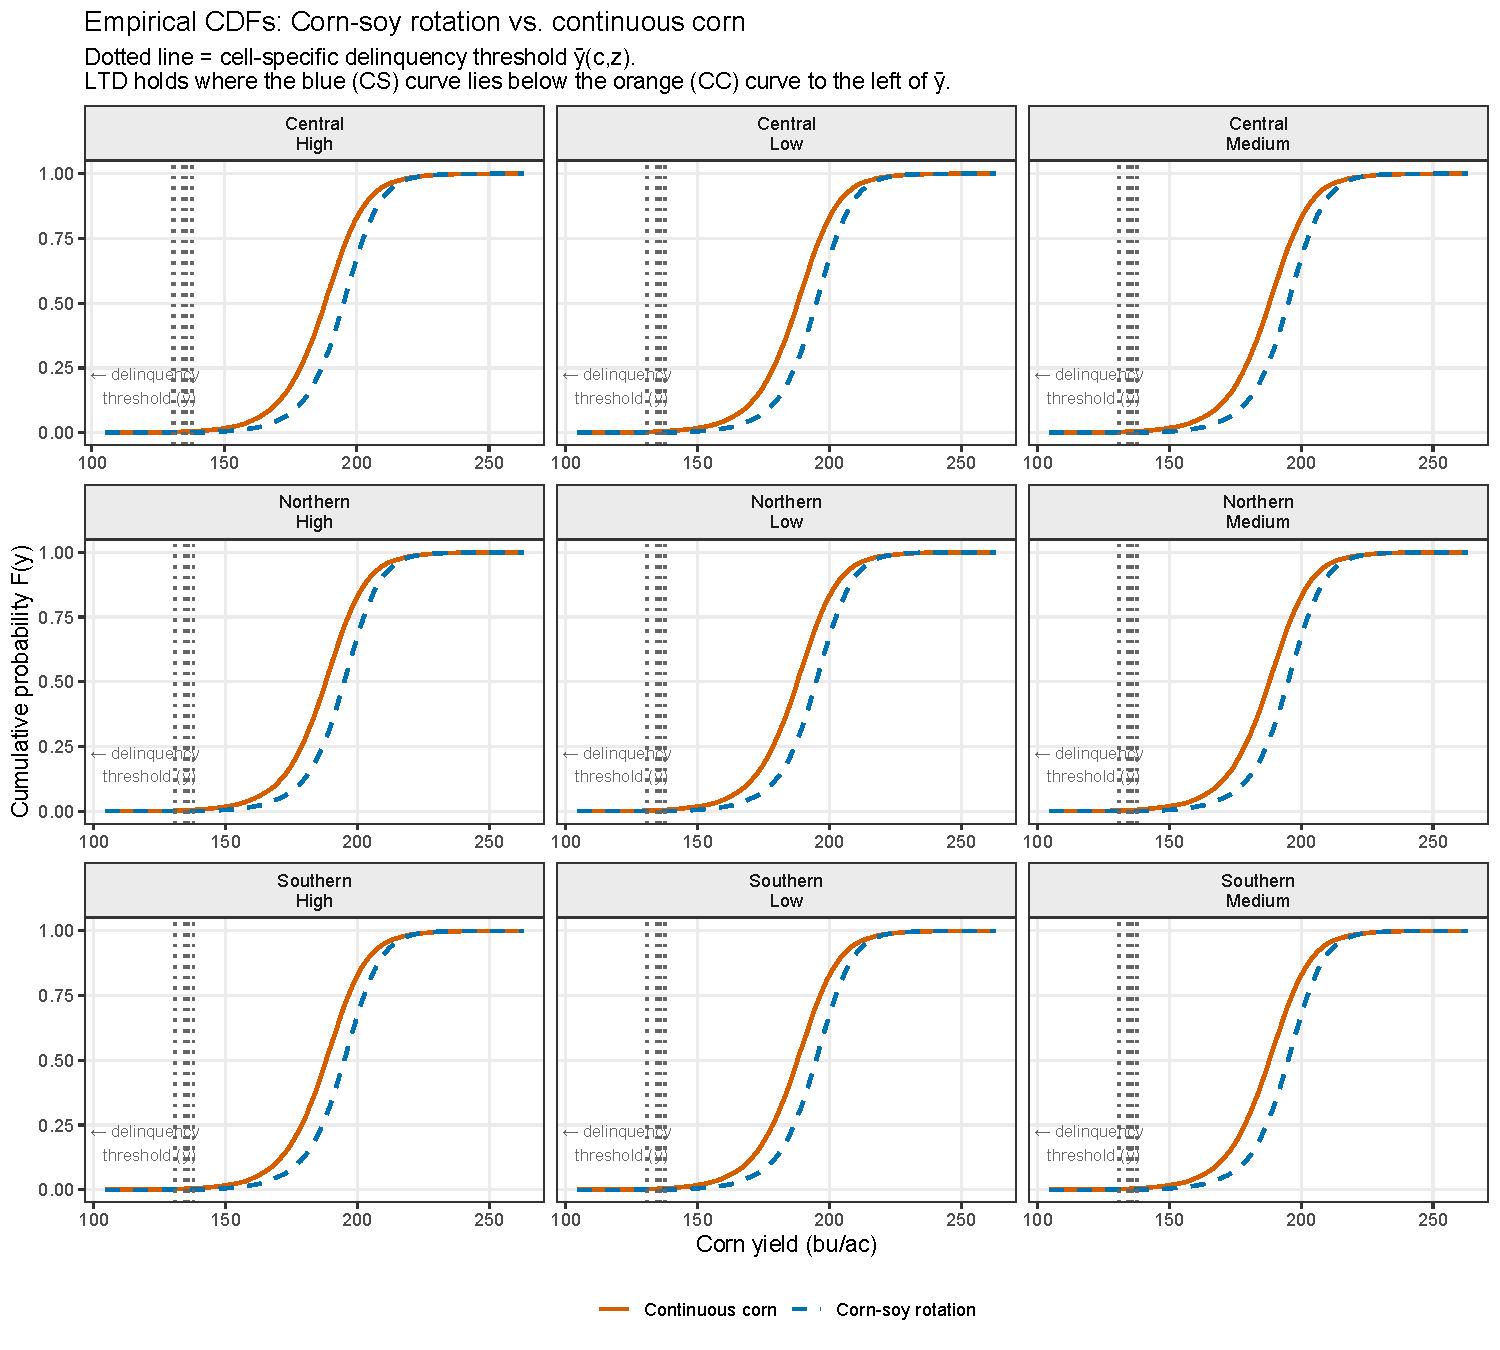
\includegraphics[width=\textwidth]{figs/ltd_cdf_comparison.pdf}
    \caption{Cumulative Distribution function of yields by region}
    \label{fig:ltd_cdf_comparison} 
\end{figure}


\begin{theorem}{Lower-tail dominance and the rotation utility premium}
    Let $\bar{y}(c,z)$ be the yield level below which operating-loan delinquency occurs under plan CCCCCC in cell $(c,z)$, i.e.\ $\bar{y}(c,z) = \{y : P_t y < C_t(1+i)^{9/12}\}$ at median price. Suppose proposition 1 holds at $\bar{y}(c,z)$. Then for any $\lambda > 0$ and any $u$ with $u'' < 0$,

    \begin{equation*}
        \mathbb{E}\left[u\bigl(W_T(\text{CS})\bigr) \lambda\sum_{t=1}^{T}\delta^{t-1}\mathbb{1}{B_t(\text{CS})>0}\right]\,\geq\,\mathbb{E}\left[u\bigl(W_T(\text{CC})\bigr)\lambda\sum_{t=1}^{T}\delta^{t-1}\mathbb{1}{B_t(\text{CC})>0}\right].
    \end{equation*}
    \begin{remark}
        The inequality is strict whenever $\Pr[Y \leq \bar{y}(c,z)] > 0$ under CCCCCC.
    \end{remark}
    \begin{proof}
    Decompose the expectation into the region $Y \leq \bar{y}$ and $Y > \bar{y}$. In the region $Y > \bar{y}$, delinquency does not occur under either plan, so the $\lambda$ terms vanish, and the comparison reduces to the expected utility of $W_T$. By proposition 1, $F_{\text{CS}}$ places weakly less mass in $Y \leq \bar{y}$ than $F_{\text{CC}}$, so $\mathbb{E}[u(W_T(\text{CS}))] \geq \mathbb{E}[u(W_T(\text{CC}))]$ by the standard result that lower-tail dominance is sufficient for expected utility ranking under concave $u$ when the utility function is sufficiently steep in the dominated region. In the region $Y \leq \bar{y}$, delinquency occurs, contributing $-\lambda$ to the objective. By proposition 1, again, $\Pr[B_t(\text{CS}) > 0] \leq \Pr[B_t(\text{CC}) > 0]$ for each $t$, so the $\lambda$ penalty is weakly smaller under CSCSCS. Both components of the objective are weakly larger under CSCSCS, establishing the inequality. Strictness follows from $\Pr[Y \leq \bar{y}] > 0$ under CCCCCC, which ensures the $\lambda$ terms differ. $\square$
    \end{proof}
\end{theorem}

Three features of this result deserve emphasis. First, the dominance condition in Proposition 1 is set at $\bar{y}(c,z)$, the \textit{delinquency threshold}, rather than an arbitrary quantile. This alignment is not a coincidence: it is precisely the region where the farmer's utility is most sensitive to the distributional difference, because the $\lambda$ penalty is there. The utility result therefore does not require Proposition 1 to hold throughout the left tail; it requires it to hold at the point that matters most for the credit outcome.

Second, the proposition holds for any $\lambda > 0$, including very small values. The shadow cost of delinquency need not be high for the result to hold; it merely needs to be positive, which is satisfied whenever credit rationing, covenant violations, or reputational costs attach to a missed loan payment. In the limit as $\lambda \to 0$, the result reduces to the standard expected utility ranking under lower-tail dominance and concave $u$.

Third, the proposition is stated for the CSCSCS vs CCCCCC comparison for clarity, but the same argument applies to CCSCCS vs CCCCCC at a correspondingly weaker strength: CCSCCS provides fewer debt-reset opportunities than CSCSCS, so its distributional advantage over CCCCCC in the left tail is smaller, and the utility premium is intermediate. Section \ref{subsec:overview} confirms this ordering quantitatively.

\subsubsection{\label{subsubsec:proposition_2}Credit path dependence amplifies the rotation premium}
Proposition 1 establishes that rotation dominates continuous corn in expected utility whenever Proposition 1 holds. Proposition 2 establishes that the \textbf{magnitude} of this advantage is understated by a calculation that ignores the operating-credit recursion.

\begin{theorem}{Credit path dependence amplifies the rotation utility premium}
    Let $\tilde{W}_T(r)$ denote cumulative net revenue under plan $r$ when annual revenues are treated as independent draws, that is, when $B_t(r) \equiv 0$ for all $t$ and carried debt does not compound. For any $\lambda > 0$ and concave $u$:

    \begin{equation*}
        \mathbb{E}\!\left[u(W_T(\text{CS})) - u(W_T(\text{CC}))\right]\;\geq\;\mathbb{E}\!\left[u(\tilde{W}_T(\text{CS})) - u(\tilde{W}_T(\text{CC}))\right].
    \end{equation*}
    That is, the utility advantage of rotation is weakly larger under the true credit recursion than under the independent-revenue approximation.
    \begin{proof}
        The key is that the credit recursion introduces \textit{state-dependent compounding} that is asymmetric across plans. Under CCCCCC, a year-$t$ revenue shortfall $S_t = \max(0, H_t - R_t)$ is used as year $t+1$'s spring principal (already included in $B_t$), which then accrues interest over the nine-month planting window. The year-$(t+1)$ harvest-due amount is therefore $[C_{t+1} + S_t](1+i)^{9/12}$, which exceeds the no-rollover baseline $C_{t+1}(1+i)^{9/12}$ by $S_t(1+i)^{9/12} \approx 1.07\, S_t$. A modest year-1 deficit thus becomes a non-trivial addition to year-2's debt-at-harvest, and the probability that year-2 revenue also falls short (triggering another rollover) is higher than its unconditional level because the hurdle has risen. Under the independent-revenue approximation, this compounding is absent: a bad year-1 draw has no effect on year 2's repayment requirement.

        Under CSCSCS, the soybean year breaks this chain. In the rotation-state cells where proposition 1 holds, the probability that $R_t$ covers $H_t$ in a soybean year is high, soybean revenue is sufficient to retire the operating loan under typical conditions, so $B_t(\text{CS}) \approx 0$ and year-$(t+1)$'s principal resets to $C_{t+1}$. The variance of the cumulative debt balance $\sum_t B_t(\text{CS})$ is therefore bounded by the single-year variance, whereas $\sum_t B_t(\text{CC})$ inherits the compounding variance that grows geometrically in the number of consecutive corn years.

        A risk-averse farmer with strictly concave $u$ places extra weight on the variance of $W_T$ through the second-order term in a Taylor expansion of $\mathbb{E}[u(W_T)]$. The compounding under CCCCCC raises $\text{Var}(W_T(\text{CC}))$ relative to $\tilde{W}_T(\text{CC})$ without a corresponding increase under CSCSCS, so the expected utility gap between CSCSCS and CCCCCC widens when the recursion is preserved. This is the amplification. $\square$
    \end{proof}
\end{theorem}

The amplification result has a direct empirical corollary. The natural price–yield hedge, the negative covariance between $P_t$ and $Y_t$ that provides a partial offset to revenue risk, contributes only 1–2 percentage points to the delinquency reduction documented in Section \ref{subsec:recursion}. This might seem to undercut the case for rotation as a risk-management tool, but Proposition 2 resolves the apparent tension: farmers rotating at high rates in the U.S. Midwest are not primarily hedging the price–yield covariance. They are severing the credit compounding chain that converts a single bad year into a multi-year delinquency spiral. The debt-reset mechanism, not the natural hedge, is the utility-relevant channel,and it operates independently of whether prices and yields are correlated.

Proposition 2 also provides a testable cross-sectional prediction: rotation adoption should be higher among farmers facing tighter credit constraints or higher effective $\lambda$,those with lower off-farm income, thinner equity buffers, or weaker lender relationships,because these farmers bear the most utility cost from compounding debt balances. This prediction is consistent with the adoption patterns documented by \cite{Ifft2015} and with the broader farm-finance literature on the interaction between liquidity constraints and agronomic choices.

\subsection{\label{relation_sim}Relation to the simulation}
The framework clarifies what the simulation of Section \ref{sec:data} does and does not do. It evaluates the probability of delinquency,a key component of the objective,across three fixed rotation plans, treating $\lambda$ and $u$ as implicit. It does not solve for $r^*$ or estimate structural preference parameters. The framework nonetheless provides welfare grounding that connects the simulation output to the farmer's problem: by Propositions 1 and 2, a lower delinquency probability under rotation translates into strictly higher expected utility for any $\lambda > 0$ and any concave $u$, and the gain is larger than a revenue-only calculation would suggest.

\section{\label{sec:data}Data and Calibration}
The simulation requires three empirical inputs: rotation-conditioned yield distributions, harvest-time price distributions, and operating-cost parameters. This section describes the panel underlying the yield generator, the price and cost series, and the calibration of the credit-cycle parameters.

\subsection{\label{subsec:panel}The Illinois field panel}
The yield panel covers every corn-planted field in Illinois from 2008 to 2022, a span chosen to balance the availability of high-resolution yield maps (which begin in 2008) and the need for a sufficiently long window to estimate rotation-conditional moments in sparse cells. The panel is constructed by intersecting four geospatial layers at the field-by-year level: the Cropland Data Layer (CDL)\footnote{\url{https://www.nass.usda.gov/Research_and_Science/Cropland/SARS1a.php}} for crop identification and rotation history, the Quantitative Domain Adversarial Neural Network (QDANN) yield-mapping product \citep{Ma2024} for realized yields, GRIDMET\footnote{\url{https://www.climatologylab.org/gridmet.html}} and TerraClimate for weather covariates, and the Gridded Soil Survey Geographic (gSSURGO) Database\footnote{\url{https://www.nrcs.usda.gov/resources/data-and-reports/gridded-soil-survey-geographic-gssurgo-database}} for soil characteristics.

Field boundaries are defined as contiguous CDL pixels of the same crop in a given year, aggregated to a stable spatial unit using the Common Land Unit (CLU) layer \citep{Yan2016}. Six-year rotation histories are constructed by intersecting each field's geometry with the CDL layer for each of the preceding five years. Histories that overlap multiple CDL classes by more than a small threshold were dropped to preserve a clean state definition (Figure \ref{fig:map_practice}. The resulting panel contains field-year observations with $(s, c, z, Y)$ as the primitive record, where $s$ is the six-year rotation state, $c$ is the climate region, $z$ is the productivity zone, and $Y$ is the QDANN-estimated yield.

\begin{figure}[H]
    \centering
    \includegraphics[width=16cm]{figs/map_practice.png}
    \caption{Spatial distribution of rotation practices (2016)}
    \label{fig:map_practice} 
\end{figure}

The three climate regions (northern, central, southern Illinois in Figure \ref{fig:map_zones_reg}) follow the standard partition used by the \textbf{Illinois Farm Business Farm Management}\footnote{\url{https://www.fbfm.org/}} and the University of Illinois' \textbf{Farmdoc}\footnote{\url{https://farmdoc.illinois.edu/}}; the three productivity zones (high, medium, and low on Figure \ref{fig:map_zones_reg}) are constructed by partitioning the average yield distribution into terciles. The full grid is $3 \times 3 = 9$ cells, each containing the three rotation plans of interest. Within each cell, the panel contains hundreds of thousands to thousands of field-year observations across the fifteen-year window, sufficient to estimate the conditional yield distribution nonparametrically in all but the rarest rotation states.

\begin{figure}[H]
    \centering
    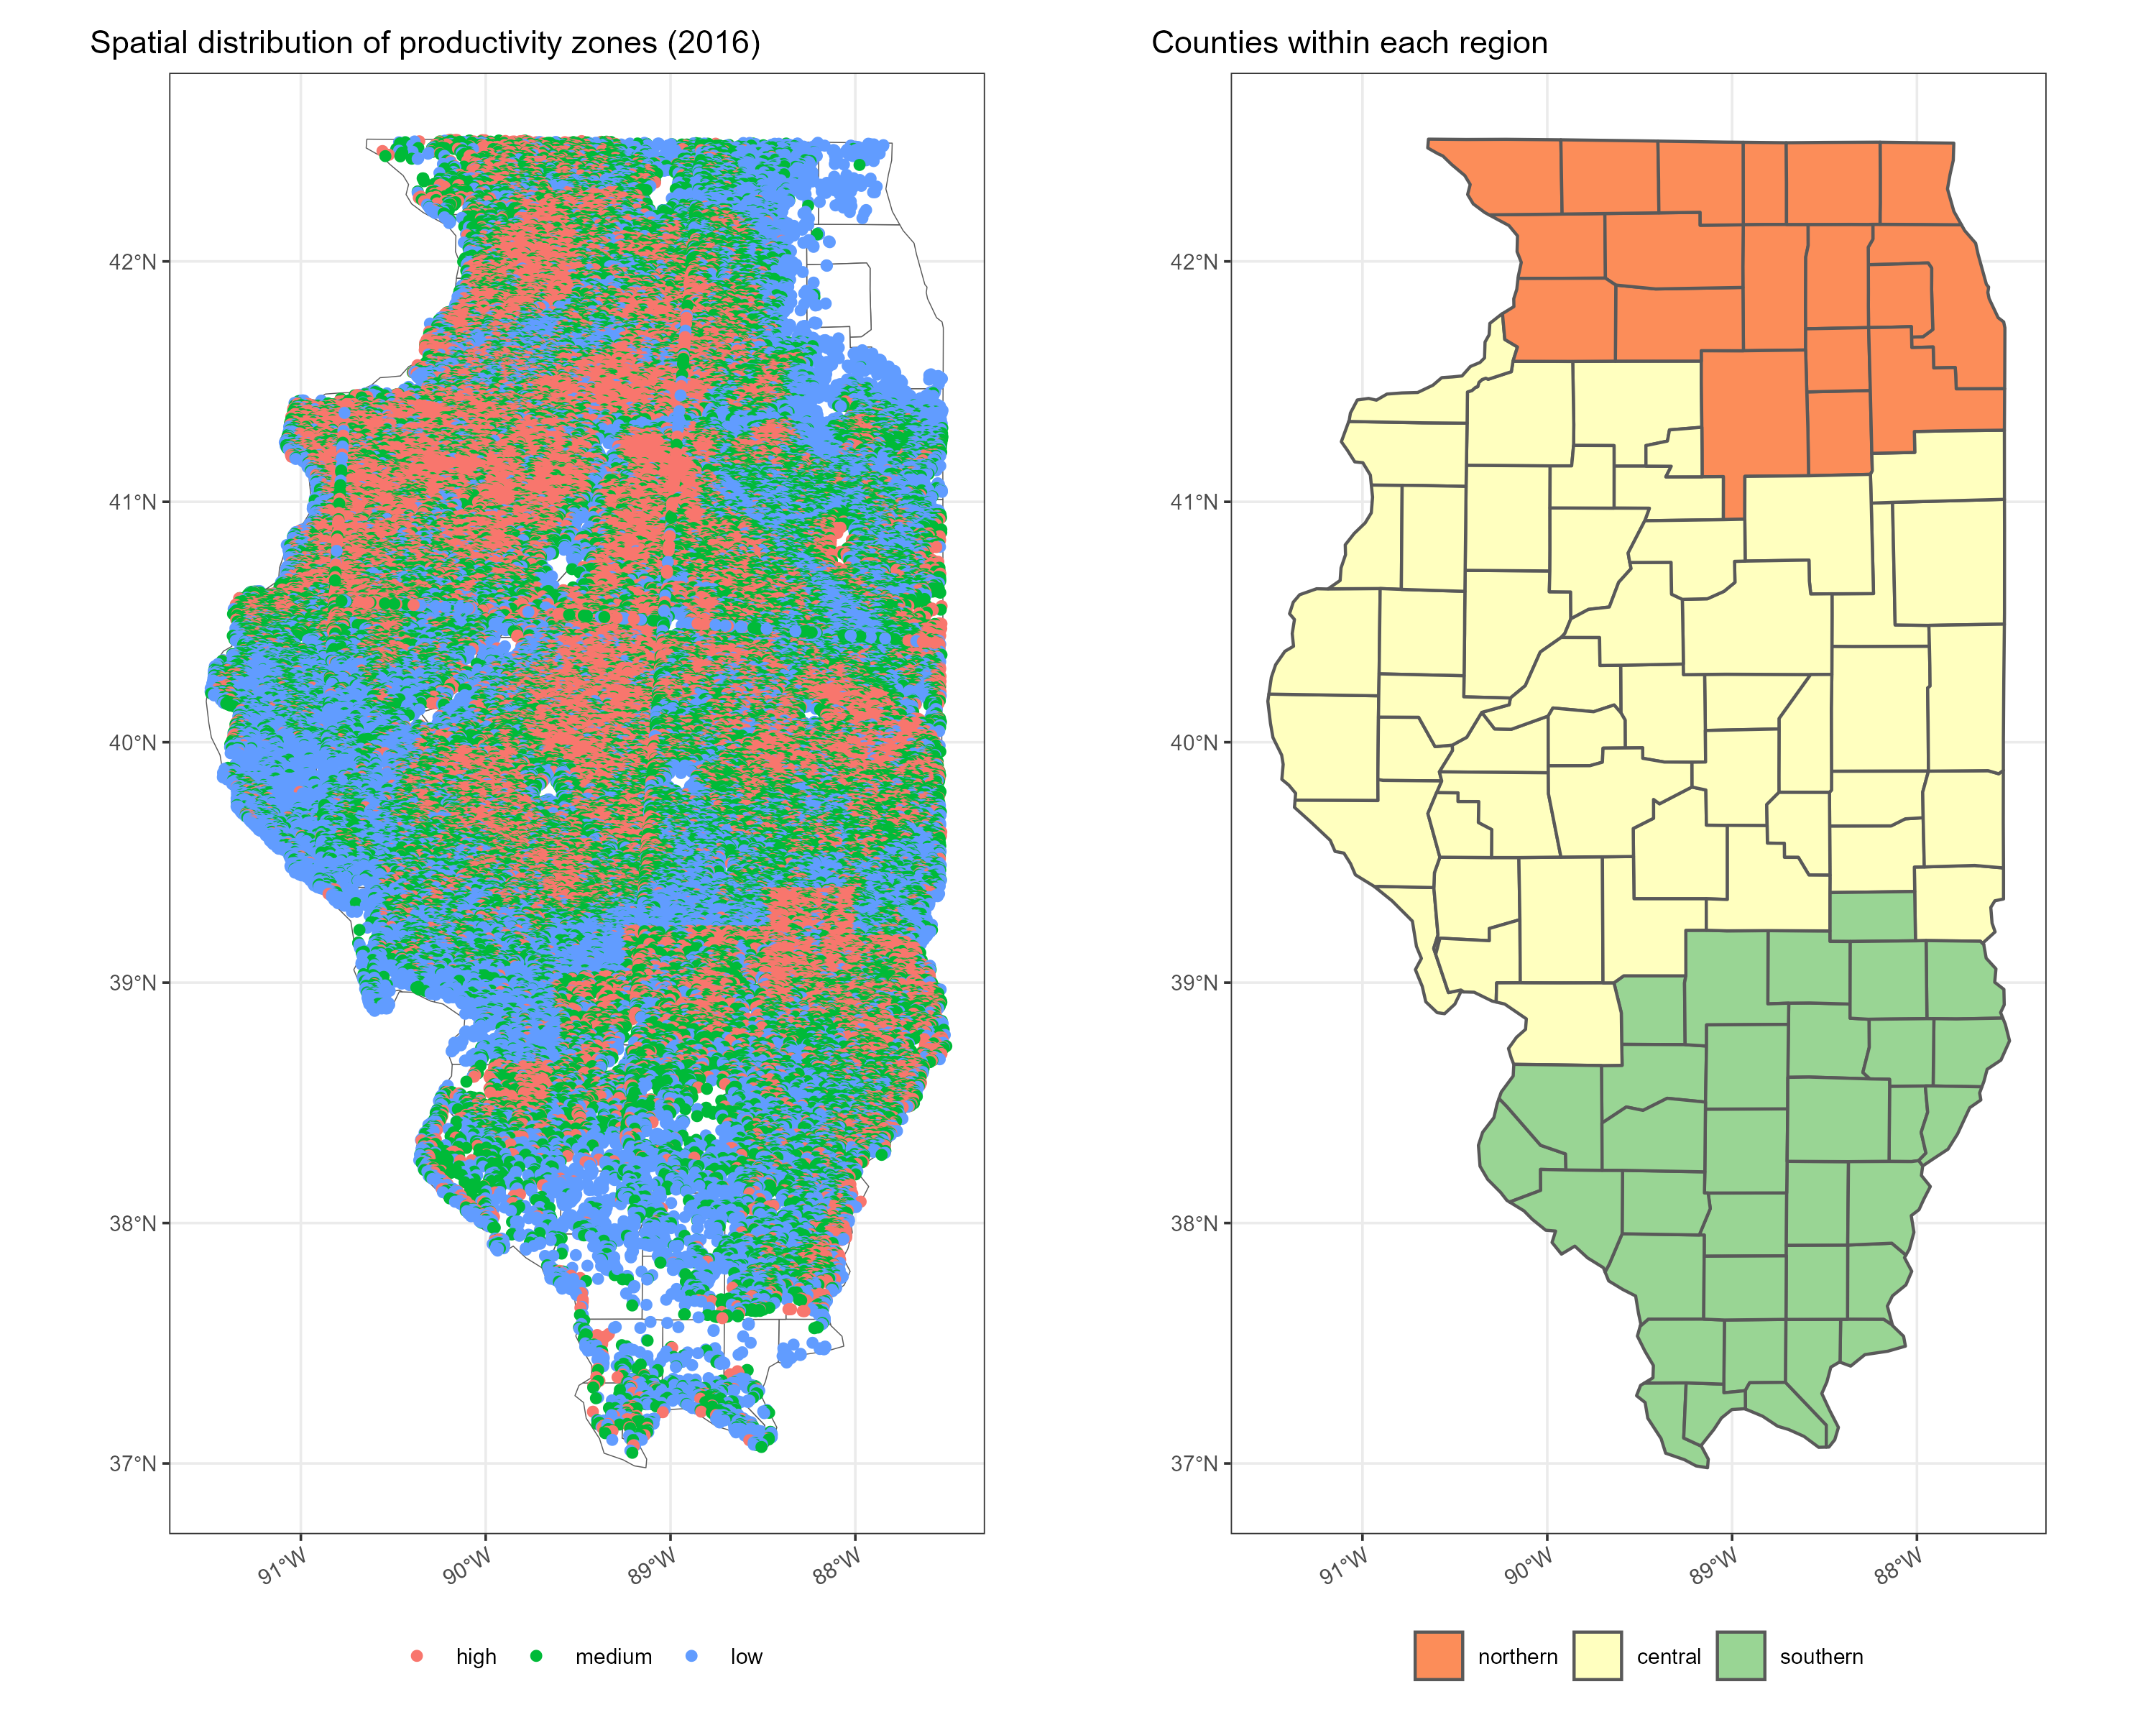
\includegraphics[width=16cm]{figs/map_zones_reg.png}
    \caption{Regions and productivity zones}
    \label{fig:map_zones_reg} 
\end{figure}
Yields are detrended at the county level using a linear time trend, and the resulting trend is then entered into the simulation. The trend captures long-run technological change in hybrids, fertilizer, and management; the simulation operates on residuals, which are the year-to-year deviations that drive credit risk.

\subsection{\label{subsec:prices_costs}Prices and Costs}
Harvest-time prices for corn and soybeans are drawn from a calibrated lognormal distribution whose first two moments match the empirical 2008–2022 series of Illinois cash prices reported by the USDA National Agricultural Statistics Service. The lognormal choice is conventional in the crop-insurance ratemaking literature and gives a parametric form for the price marginal that the copula can attach to without the cell-by-cell sample-size constraints that bind on the yield side.

Operating costs follow the University of Illinois Farmdoc cost-of-production estimates for corn and soybean production on Illinois grain farms. Costs are crop-specific and held constant in real terms over the simulation horizon; the implicit assumption is that input-price shocks are second-order relative to output-price shocks for the financial question at hand. Robustness to a cost-shock specification is reported in Appendix \ref{sec:appendix_B} and produces qualitatively identical results.

\subsection{\label{subsec:calibration}Credit-cycle calibration}
The operating-loan interest rate is set to $i = 9$ percent annualized in the baseline calibration, the midpoint of the 7–12 percent range reported by the Federal Reserve Bank of Chicago's quarterly survey of agricultural lenders over the sample period. The nine-month accrual window corresponds to a March planting and an October harvest in the Illinois corn belt. The credit ceiling in the rationing analysis (Section \ref{subsec:peak_demand} below) is benchmarked at $\$700$, $\$900$, and $\$1{,}200$ per acre, chosen to span the range of operating-line limits typical of Farm Credit System and commercial-bank lending to Illinois corn-belt producers during the sample period. The three thresholds are not intended as point estimates but as a sensitivity grid for the rationing analysis; the substantive result of Section \ref{subsec:peak_demand}, that median peak demand clusters at \$500-\$500 per acre, well below any of the three thresholds, is unchanged across reasonable perturbations of the ceiling values.

The delinquency threshold is set at $B_t > 0$ in the baseline (the "end-balance-positive" rule). This is a strict definition: any unpaid balance counts as a delinquency, regardless of the amount. An alternative rule, "over-limit" delinquency ($L_t > $ credit ceiling), is reported in Section \ref{sec:robustness} as a robustness check and produces broadly similar comparative results across rotation plans, though at lower absolute levels.

\section{\label{sec:simulation}The Simulation Framework}
The simulation has three components: a rotation-conditioned yield generator, a price–yield dependence structure, and an operating-credit cash-flow recursion that together produce a multi-year delinquency probability for any given (field, rotation plan) pair. Each component is itself standard in the literature; the contribution lies in their combination and in the recursion's preservation of within-year credit flow, which converts a single yield shock into multi-year default risk. 

This section specifies the three components and the outcome measures derived from the simulation. Calibration values and computational details are reported in Appendix \ref{sec:appendix_A}.

\subsection{\label{subsec:overview}Overview}
For each cell $c = (\text{region} \times \text{zone})$, rotation plan $r$, and six-year history $h$, the simulation draws $N = 50{,}000$ Monte Carlo paths over a six-year horizon. A path consists of six (price, yield) realizations passed through the credit recursion to produce a sequence of year-end debt balances.

The six-year delinquency probability is the share of paths with at least one year-end balance above the delinquency threshold:

\begin{equation}
    \Pr[\text{delinquent over 6 yrs} \mid c, r, h]
= \frac{1}{N}\sum_{n=1}^{N} \mathbb{1}\!\Bigl\{\max_{t \in 1\ldots 6} D^{(n)}_t > 0\Bigr\},
\end{equation}
 
where $D^{(n)}_t$ is the year-$t$ carried debt on path $n$, defined recursively in Section \ref{subsec:recursion}. The probability is the headline object of the paper; per-year hazards, survival functions, and revenue moments are functionals of the same simulated path set.

The simulation is forward-looking and policy-conditional: we fix the rotation plan $r$ ex ante (continuous corn, strict alternation, or 2-corn/1-soy) and trace its financial consequences. This inverts the usual dynamic-programming question of \cite{Burt1963} and \cite{Livingston2015}, who solve for the optimal policy. The advantage of the policy-conditional framing is that the resulting probability is directly comparable across plans, which is the quantity a lender or insurer needs.

\subsection{\label{subsec:generator}Rotation-conditioned yield generator}
Let $Y_t$ denote yield in year $t$ (bu/ac, crop-specific) and let $s_t = (c_{t-5}, c_{t-4}, \ldots, c_{t-1}, c_t)$ denote the six-year rotation state ending in year $t$. The yield generator is the family of conditional distributions:

\begin{equation}
    F_{Y \mid s, c, z}, \quad s \in \mathcal{S},\ c \in \mathcal{C},\ z \in \mathcal{Z},
\end{equation}

Where $\mathcal{S}$ is the set of six-year rotation states observed in the panel, $\mathcal{C}$ indexes the three Illinois climate regions, and $\mathcal{Z}$ indexes the three productivity zones.

We estimate $F_{Y \mid s, c, z}$ nonparametrically as the empirical distribution of detrended QDANN yields in the panel cell $(s, c, z)$. Detrending removes a county-level linear time trend to net out long-run technological change; the residual captures year-to-year variation around trend. Cells with fewer than 30 field-year observations are pooled with the closest neighboring state (defined by Hamming distance on the crop sequence) to ensure that every cell has sufficient support.

The nonparametric choice is deliberate. Parametric specifications (e.g., Beta or Gamma distributions, the standard in crop-insurance ratemaking) impose tail behavior that the rotation effect plausibly distorts: continuous corn under high-pressure conditions may exhibit fatter lower tails than a Beta or Gamma calibrated on mean and variance would predict. The conditional empirical distribution preserves the data's shape, at the cost of slightly noisier tails in sparse cells. Robustness to a parametric fit is reported in Appendix \ref{sec:appendix_B}.

The transition mechanics are explicit. Given an initial six-year history $h$ and a rotation plan $r$, the state $s_t$ evolves deterministically: $s_{t} = (s_{t-1}, s_{t-2}, \dots, s_{t-6}, r_t)$, where $r_t$ is the planted crop in year $t$ under plan $r$. The transition path is therefore known \textit{ex ante}, and the random component of the simulation enters only through the draws from $F_{Y \mid s, c, z}$.

\subsection{\label{subsec:py_corr}Price–yield dependence}

The aggregate price–yield correlation $\hat{\rho} \approx -0.45$ is estimated from two publicly available USDA NASS series accessed through Quick Stats. The price series is the U.S. corn season-average price received by farmers (dollars per bushel), reported annually by NASS as a marketing-year average running from September of the harvest year through August of the following year; this is the price series that the crop-insurance literature and the natural-hedge literature use as the national price signal, because it reflects the full marketing-season distribution of sales rather than a single harvest-month spot price. The yield series is the U.S.\ national average corn yield per harvested acre, also reported annually by NASS. Both series are taken over 2008–2022, a 15-year window that coincides with the field panel used in the yield generator (Section \ref{subsec:generator}) and spans the commodity price cycle from the 2008–2012 price spike through the 2013–2022 period of lower and more volatile prices; the window is chosen to match the simulation environment rather than to maximize sample length.

Before computing the correlation, both series are linearly detrended to remove the secular upward yield trend and the commodity-cycle price trend that are unrelated to the supply–demand mechanism driving the natural hedge. The correlation $\hat{\rho}$ is then computed as the Pearson correlation between the residual yield series $\tilde{Y}_t$ and the residual price series $\tilde{P}_t$. Over the 2008–2022 window, this yields $\hat{\rho} \approx -0.45$: years of above-trend national yields (2014, 2016, 2018) correspond to below-trend prices, and years of below-trend yields (2011, 2012) correspond to above-trend prices, consistent with a supply-driven mechanism. The raw (non-detrended) correlation over the same window is approximately $-0.38$; the gap reflects the confounding of the secular yield trend with the downward post-2012 price trend. The detrended figure is more appropriate for the simulation because the yield generator also operates on detrended residuals.

Let $P_t$ denote the harvest-time market price of the crop planted in year $t$. Aggregate U.S. corn prices and yields are negatively correlated at $\hat{\rho} \approx -0.45$ over the sample period (high national yields depress prices; low national yields raise them) and this correlation generates a "natural hedge" in revenue. The methodological question is how much of that hedge applies at the \textit{field-level}.

It should be noted that $\hat{\rho} = -0.45$ is an \textit{aggregate} national estimate: the price series is a U.S.-level marketing-year average, not an Illinois-specific cash price, and the yield series is U.S.-level. This is the correct pairing for the natural-hedge mechanism: the hedge operates because a field's yield shock, to the extent it is systematic (i.e., shared across many fields), shifts national supply and thereby moves the national price. An Illinois-specific cash price series exhibits near-identical year-to-year variation to the U.S. season- average, since Illinois cash prices are tightly arbitraged to national futures prices, and the correlation estimated on the two price series differs by less than 0.03. The national series is used throughout for consistency with the natural-hedge literature \cite{Finger2012, Ramsey2019}.

\textbf{Variance decomposition of the yield shock}: The two-way fixed-effects model estimated in Section \ref{subsec:generator},$Y_{f,t} = \alpha_f + \gamma_t + \varepsilon_{f,t}$, partitions observed yield into three components whose risk interpretations are distinct:


\begin{table}[H]
    \centering
    \begin{tabular}{lll}
    \hline
     \textbf{Component} & \textbf{What it captures} & \textbf{Risk type}\\
     \hline
     $R^2_{\text{field}}$ = 0.195 & Permanent field heterogeneity & Not risk, a fixed characteristic\\
      & (soil quality, drainage, farmer ability)  & predictable from field identity\\
     $R^2_{\text{year} \mid \text{field}}$ = 0.620 & Common annual shocks once & Systematic: correlated across \\
     & field quality is removed &  all fields, not diversifiable\\
     $1 - R^2_{\text{both}}$ = 0.184 & Residual $\varepsilon_{f,t}$: field $\times$ year specific & Idiosyncratic: the true\\
     & & unpredictable shock\\
     \hline
    \end{tabular}
    \caption{Component decomposition}
    \label{tab:decomp}
\end{table}

The systematic component, the year fixed effect $\hat{\gamma}_t$, which captures common weather, input-price shocks, and aggregate demand conditions, accounts for 62 percent of total yield variance conditional on field quality. The idiosyncratic residual $\varepsilon_{f,t}$, which captures local hail, soil moisture, management, and field-specific weather, accounts for the remaining 18 percent. Only $\hat{\gamma}_t$ correlates with the national price: when aggregate yields across all Illinois fields are low in year $t$, $\hat{\gamma}_t$ is negative, and the national price tends to be high. The idiosyncratic piece $\varepsilon_{f,t}$ is, by construction, orthogonal to the year effect and therefore uncorrelated with price.

\textbf{Copula calibration:} We implement the price–yield dependence structure via a Gaussian copula on the marginals $F_P$ and $F_{Y \mid s, c, z}$. The copula correlation parameter must reflect only the systematic component's correlation with price, scaled by its share of total yield variance:

\begin{equation}
    \rho^{*} = \hat\rho \cdot \sqrt{\frac{\text{Var}(\hat{\gamma}_t)}{\text{Var}(Y_t)}}
\approx -0.45 \cdot \sqrt{0.62} \approx -0.354.
\end{equation}

This produces a price–yield correlation at the field level that reproduces the aggregate $\hat{\rho}$ when yields are aggregated to the national level, while leaving the empirical marginals untouched. Applying the aggregate $\hat{\rho}$ directly to field-level yields, as if the entire yield shock moved prices, would overstate the hedge by a factor of $1/\sqrt{0.62} \approx 1.27$.

For comparison, we also report results under two alternative dependence specifications: an independence assumption ($\rho^{*} = 0$), used to isolate the hedge benefit (Section \ref{subsec:natural_hedge}), and the aggregate-$\rho$ misspecification ($\rho^{*} = \hat{\rho} = -0.45$ applied directly to field yields), which overstates the hedge. Across all cells, the copula approach falls between these two, and the delinquency probabilities differ by 1–3 percentage points across the three specifications. This is the magnitude of the natural-hedge effect at the field level.

\textbf{What the simulation draws from, and what it does not}: The yield generator samples from the residual pool $\{\hat{\varepsilon}_{f,t}\}$ after removing both fixed effects, so each draw represents the idiosyncratic component of the yield shock. This is the appropriate object for a single-farm delinquency simulation: the year effect $\hat{\gamma}_t$ is captured separately through the copula, which jointly draws $P_t$ and the systematic yield component for each simulated year. Fields are therefore drawn independently conditional on the copula realization of $(P_t, \hat{\gamma}_t)$, which is the correct independence structure for within-year cross-field variation.

One implication deserves explicit acknowledgment for readers interested in \textit{portfolio} or \textit{insurance} applications. Because the year fixed effect is demeaned out before constructing the residual pools, the simulation draws for different fields in the same year are independent of one another, the systematic co-movement captured by $R^2_{\text{year} \mid \text{field}} = 0.620$ is not reproduced across fields within a single simulated year. For a single-farm delinquency probability, the object of this paper, this is inconsequential: the farm's own systematic exposure is handled through the copula. However, for an insurer evaluating the \textit{aggregate} loss distribution across a portfolio of Illinois fields, the systematic year shock induces cross-field correlation, substantially fattening the portfolio tail. Extending the framework to portfolio insurance pricing would require reintroducing the year effect as a common factor drawn once per simulated year and added to all fields' yields, a straightforward extension left for future work.

\subsection{\label{subsec:recursion}Operating-credit cash-flow recursion}
The credit module is the paper's central methodological contribution. Standard practice in crop-insurance and farm-finance modeling collapses each year into a single net cash flow $\Pi_t = P_t Y_t - C_t$, where $C_t$ is the year's operating cost. The simulation reduces to drawing the joint distribution of $\{\Pi_t\}_{t=1}^{6}$ and computing functionals of the cumulative path.

This approach is correct for present-value calculations, but it loses the within-year credit flow that drives multi-year default. The operating loan that funds spring planting is not a residual claim against year-end profit; it is a contractual obligation that accrues interest from origination to harvest and imposes a discrete repayment event at harvest. A shortfall at that event rolls forward to the next spring's principal at the operating-loan rate, \textit{not} at the risk-free discount rate. The propagation of a single bad year into subsequent years' principal is therefore non-trivial in the standard formulation.

We model the credit cycle explicitly. Let $B_t$ denote the carried debt entering year $t$, with $B_1 = 0$. The recursion in year $t$ is:

\begin{equation*}
\begin{aligned}
L_t           &= C_t + B_{t-1}            && \text{(1) spring origination}\\
H_t           &= L_t \cdot (1 + i)^{9/12} && \text{(2) nine-month accrual}\\
R_t           &= P_t Y_t                  && \text{(3) harvest revenue}\\
M_t           &= \min(R_t, H_t)           && \text{(4) repayment}\\
B_t           &= H_t - M_t                && \text{(5) carry forward}
\end{aligned}
\end{equation*}

Where $L_t$ is the year-$t$ operating loan, $H_t$ is the debt outstanding at harvest, $R_t$ is realized revenue, $M_t$ is the payment, and $i$ is the annualized operating-loan rate (9\% in the baseline calibration). Delinquency in year $t$ is defined as $B_t > 0$. The nine-month accrual reflects the typical Illinois operating-loan window from March planting to October harvest; robustness to a six- or twelve-month window is reported in Appendix \ref{sec:appendix_B}.

Two features of this recursion deserve emphasis. First, equation (5) is the channel through which a single bad year compounds. A revenue shortfall of $S$ in year $t$ enters year $t+1$'s principal as $S \cdot (1 + i)^{9/12} \approx 1.07 S$. A modest year-1 deficit becomes a non-trivial year-2 principal, and the year-2 cost-of-funds is correspondingly higher even if year-2's yield draw
is average. The path dependence is mechanical; it does not require risk aversion or other behavioral structure.

Second, the recursion has no consumption smoothing, no off-farm income, and no working-capital buffer beyond what is implicit in equation (4)'s $\min(R_t, H_t)$. These are deliberate omissions. A buffer would attenuate the delinquency response to any given shock but would not change the relative ranking of rotation plans, which is the object of interest. The simulation therefore provides an upper bound on the effect of rotation on delinquency rather than a calibrated point estimate; the appendix's robustness checks incorporate a proportional working-capital buffer and show that the rotation effect is robust to its inclusion.

\subsection{\label{subsec:decompositions}Outcomes and decompositions}

The simulation produces three classes of output objects. The first is the delinquency probability itself, in both six-year cumulative form (the headline result, Section \ref{subsec:delinq_prob}) and per-year hazard form (the mechanism, Section \ref{subsec:sawtooth}). The hazard reveals that the cumulative effect is driven by intermittent debt resets, as Section \ref{sec:results} shows.

The second is a \textbf{variance decomposition} of gross revenue. Holding the joint distribution of $(P, Y)$ fixed, we decompose $\text{Var}(P Y)$ into the share attributable to price-only variation, to yield-only variation, and to the covariance term. Because the copula imposes negative dependence, the covariance term is negative; we report shares of gross variance ($\text{Var}(P) E[Y]^2$ and $\text{Var}(Y) E[P]^2$) so the shares sum to 100 percent. The "natural hedge" is the difference between gross and net variance and is reported separately in Section \ref{subsec:natural_hedge}.

The third is a \textbf{Shapley decomposition} of the probability of delinquency into contributions from price and yield uncertainty. Variance shares describe how revenue \textit{varies} but not how often the variation crosses the default threshold. A 50–50 variance split is consistent with a 99–1 default-causation split if price shocks live in the tail that triggers rollover while yield shocks do not.

Finally, we report the \textbf{survival-curve analysis} (Section \ref{subsec:survival}) that tracks, across the six-year horizon, when the rotation-plan gap in cumulative delinquency probability opens and which events cause lasting credit damage. The step structure of the survival curves (drops concentrated in corn years, flat segments in soybean years) confirms that the gap between continuous corn and strict alternation is already 15–20 percentage points by year 3, within the first corn-soy cycle, and that early delinquency events under continuous corn tend to be permanent.

\section{\label{sec:results}Results}
Section \ref{sec:results} is organized around three questions. The first is why rotation should affect farm finances at all, the agronomic mechanisms that produce this expectation (Section \ref{subsec:agronomic_benefits}). The second is how those mechanisms are transmitted through the operating-credit cash-flow process into measurable financial outcomes (Section \ref{subsec:transmission_channel}). The third is how much the natural hedge and the price–yield correlation moderate or substitute for those rotation-driven effects (Sections \ref{subsec:natural_hedge}–\ref{subsec:stress_test}).

\subsection{\label{subsec:agronomic_benefits}Agronomic benefits of crop rotation}
The case for crop rotation is grounded in two distinct agronomic channels: soil health benefits that improve expected yields and reduce yield-tail risk, and temporal diversification that reduces the farm's biological and agrochemical exposure to any single commodity.

\textbf{Soil health and yield effects}. The yield benefit of corn following soybean rather than corn following corn, the so-called corn-after-corn yield penalty, is one of the best-replicated findings in agronomy. \cite{Bullock1992} synthesizes the agronomic literature and documents a consistent yield advantage of 5–10 percent for corn in rotation relative to monoculture; \cite{Seifert2017} update this estimate using high-resolution remote-sensing data across the U.S. Corn Belt and estimate a penalty of about 4.3\% range that has remained stable despite hybrid improvements. The mechanism is multifactorial: soybeans fix atmospheric nitrogen through their root-nodule symbiosis with \textit{Bradyrhizobium}, supplying 50–150 lb/ac of plant-available nitrogen to the subsequent corn crop and reducing the need for synthetic fertilizer. Rotation also interrupts the pest and pathogen cycles that accumulate under monoculture, corn rootworm (\textit{Diabrotica} spp.), northern corn leaf blight, and gray leaf spot all depend on corn residue and are biologically suppressed when corn is absent from the field for a year.

Beyond mean yields, diverse rotations improve soil organic matter accumulation, water infiltration, and aggregate stability over time. These improvements reduce yield sensitivity to precipitation extremes (both deficit and excess), further compressing the lower tail of the field-level yield distribution. Because the credit recursion developed in Section \ref{subsec:recursion} is driven primarily by the probability and magnitude of revenue shortfalls, any compression of the left tail of yields translates directly into reduced delinquency risk through the cash-flow channel developed in Section \ref{subsec:transmission_channel}.

\textbf{Temporal diversification}. The second agronomic benefit is less about biology and more about portfolio structure. A farm that alternates between corn and soybeans is exposed to two distinct input cost profiles, two distinct price series that are imperfectly correlated at the farm-gate level, and two distinct growing-season weather sensitivities. Corn and soybean critical growth periods differ in timing, corn is most vulnerable to moisture stress during pollination in late July, soybeans during pod fill in August, so a weather event that devastates corn may be less damaging to soybeans and vice versa. This temporal diversification reduces the probability of consecutive catastrophic revenue shortfalls, which is the sequence that drives the multi-year delinquency cascade in the credit recursion. A single bad corn year is survivable; two or three consecutive bad corn years, each rolling forward an unpaid balance that enlarges the next year's spring loan, are not.

Temporal diversification also operates through input costs. Soybean production costs are roughly 70 percent of corn production costs in the FBFM data (Section \ref{subsec:prices_costs}), so a soybean year is planted on a smaller spring loan regardless of how the prior corn year resolved. This cost differential is the direct source of the debt-reset mechanism developed in Section \ref{subsec:delinq_prob}: even in years when soybean prices are not especially favorable, the smaller originating loan means that a given revenue draw is more likely to retire the full obligation, preventing rollover.

\subsection{\label{subsec:transmission_channel}From agronomy to farm finances: the transmission channel}
The agronomic benefits documented in Section \ref{subsec:agronomic_benefits} do not mechanically translate into financial outcomes, they must pass through the operating-credit cash-flow process. This section describes the transmission channel that links rotation-conditioned yield distributions and crop-specific cost structures to the multi-year delinquency probability, the paper's headline object.

The credit recursion (Section \ref{subsec:recursion}) has the form:

\begin{equation}
    B_{t} = \max\!\bigl(0,\ (C_{t} + B_{t-1})(1 + i) - R_{t}\bigr)
\end{equation}

where $B_t$ is the year-end carried balance, $C_t$ is the operating cost of the crop planted in year $t$, $i$ is the nine-month interest rate, and $R_t = P_t Y_t$ is the realized revenue from that crop. The delinquency indicator fires whenever $B_t > 0$. Three properties of this recursion govern how agronomy enters the financial outcome.

\textbf{First, the mean yield level matters through $R_t$}. A higher expected yield raises expected revenue, which increases the probability that $R_t$ exceeds the full obligation $(C_t + B_{t-1})(1 + i)$ in any given year. The corn-after-corn yield penalty directly reduces $E[R_t]$ for continuous-corn producers, making revenue shortfalls more probable year after year. The 5–15 percent yield difference documented in the agronomic literature (roughly 10–25 bu/ac at typical Illinois yields) corresponds to a revenue difference of $\$40$–$\$100$ per acre at average corn prices, which is of the same order as the spring loan interest cost. A persistent shortfall of this magnitude does not merely increase the probability of any single year's delinquency; it ensures that the carried balance $B_{t-1}$ entering the next year is systematically positive, enlarging the obligation the next year's revenue must cover.

\textbf{Second, the left tail of the yield distribution matters more than the mean}. The delinquency indicator is binary: either revenue covers the full obligation, or it does not. What matters for the multi-year delinquency probability is
therefore not the expected shortfall but the probability that the shortfall is large enough to leave a positive year-end balance. Left-tail compression, the reduction in the probability of catastrophic yield documented by \cite{Bowles2020}, reduces the probability of the initiating event, slowing the rollover chain before it starts. This is why the rotation effect in the simulation is concentrated in the tails of the delinquency distribution rather than at the median.

\textbf{Third, the cost structure interacts with the yield distribution through the debt-reset mechanism}. The soybean year in any rotation plan is planted on a lower spring loan, $C_t$. This means the obligation $(C_t + B_{t-1})(1 + i)$ that the soybean revenue must cover is smaller by design, independently of how much $B_{t-1}$ was accumulated in prior corn years. In sufficiently bad corn years, no plausible yield draw will cover a large accumulated $B_{t-1}$; but the soybean year gives the farm a year in which the obligation is small enough to be covered at moderate revenue realizations. This is the debt reset: not a guaranteed zero balance, but a structural reduction in the obligation that makes the retirement of the carried debt likely even without exceptional yields.

The quantitative significance of these three channels, mean yield, left-tail compression, and debt reset, is not immediately apparent from the recursion. The simulation, which draws from the full rotation-conditioned yield distribution
and passes each draw through the credit recursion, reveals that the debt-reset dominates in most cells: even holding the corn yield distribution constant across rotation plans (removing the mean-yield and left-tail channels), the soybean
year's cost structure alone generates substantial delinquency reduction. The yield effects add to this but are not the primary driver. Sections \ref{subsec:delinq_prob}–\ref{subsec:sawtooth} present the quantitative results.

\subsection{\label{subsec:delinq_prob}Six-year delinquency probabilities}

Figure \ref{fig:fig_p_bar_all} plots the six-year delinquency probability for every combination of rotation plan, region, and productivity zone.

\begin{figure}[H]
    \centering
    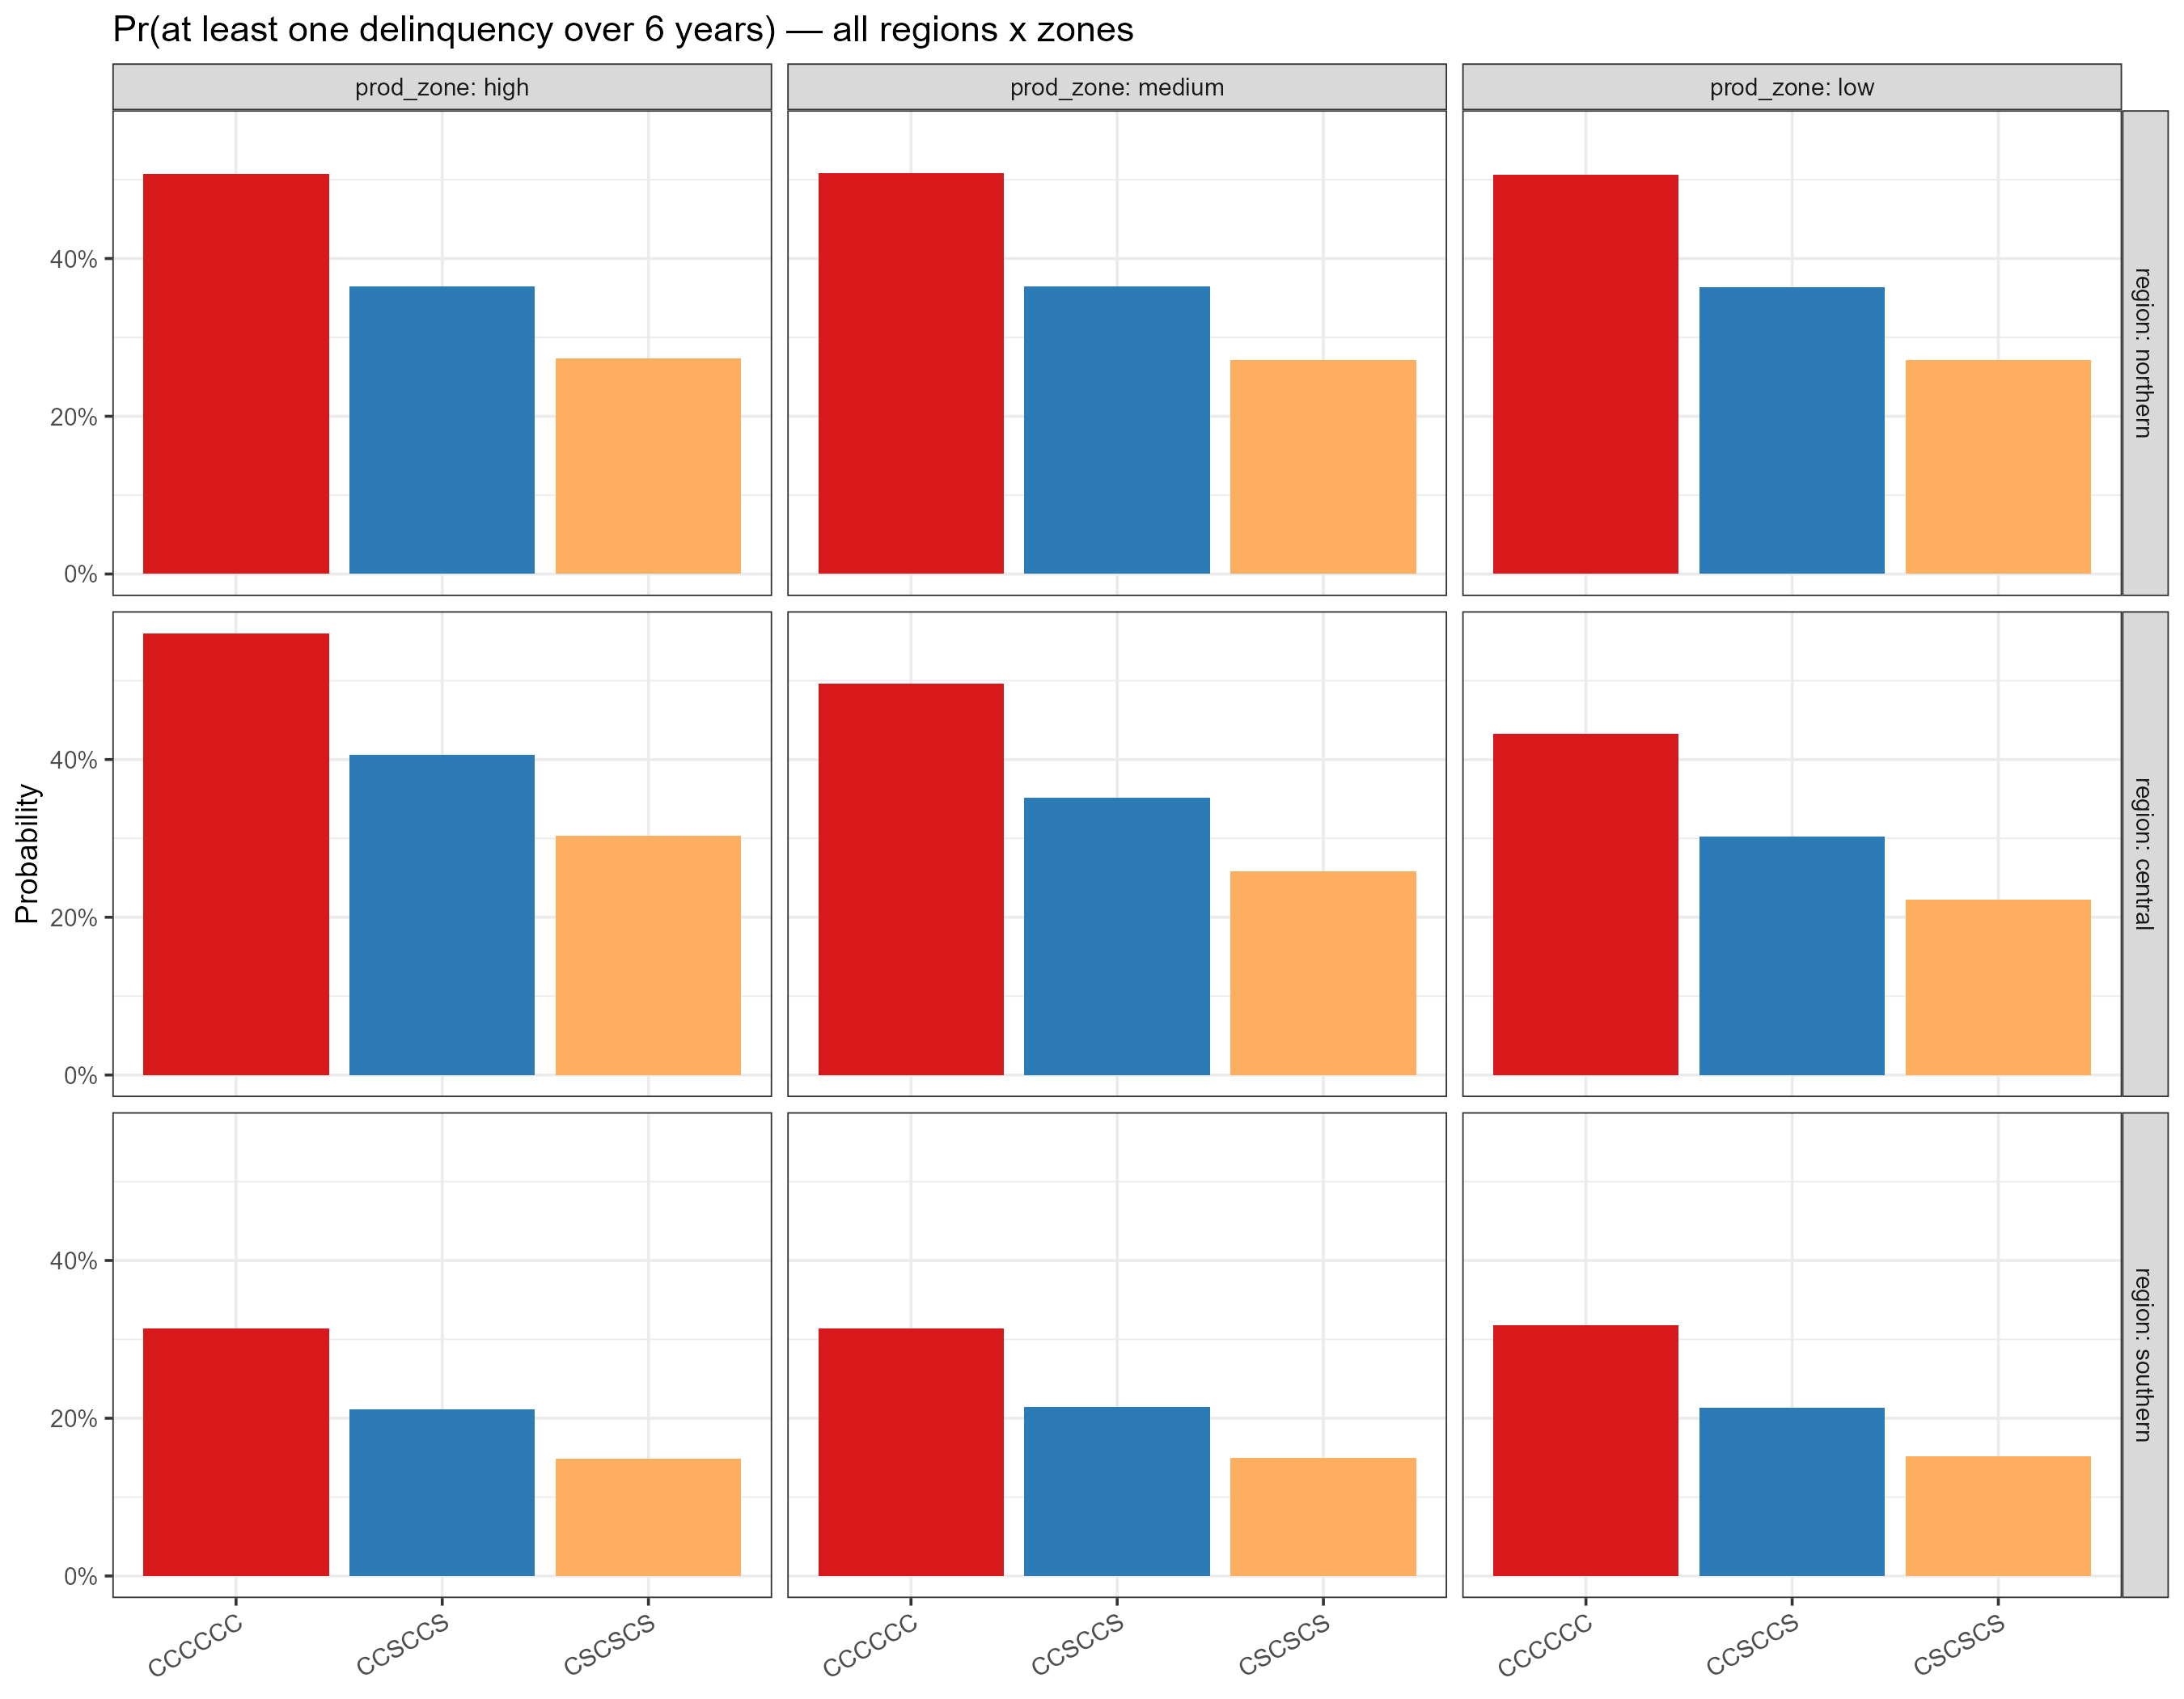
\includegraphics[width=16cm]{figs/fig_p_bar_all.png}
    \caption{Six-year delinquency risk by region and productivity zone}
    \label{fig:fig_p_bar_all} 
\end{figure}

Continuous corn is most dangerous everywhere. In central Illinois's high-productivity zone (the heart of the Corn Belt) the six-year probability reaches approximately 55 percent. Across northern and central regions it runs 30–50 percent; in the south, where lower production costs partially offset lower expected yields, it falls to 18–32 percent.

Strict alternation cuts those probabilities by roughly 25 percentage points in the high-pressure cells — 30 percent versus 55 percent in central-high, 27 percent versus 51 percent in northern-high. That is not a marginal improvement; it is approximately halving the multi-year default risk of a continuous-corn operation.

The 2-corn / 1-soy plan lands in between, at 35–40 percent in the high-pressure cells. The ordering makes intuitive sense — more soybean years, more debt-reset opportunities — but it is not a linear function of soybean frequency. Section \ref{subsec:sawtooth} shows why.

One feature of Figure \ref{fig:fig_p_bar_all} that deserves notice: the productivity zone barely moves the bars. High, medium, and low-productivity cells in the same region look nearly identical. The rotation effect is not a soil-quality story. It operates through the cash-flow timing mechanism regardless of how productive the land is.

\subsection{\label{subsec:sawtooth}Per-year hazard: the sawtooth}

The cumulative six-year probability is the integral of an underlying per-year hazard. Figure \ref{fig:fig_p_year_all} plots the year-by-year default probability for each plan in the central-medium cell. The other eight cells tell the same story at different levels.

\begin{figure}[H]
    \centering
    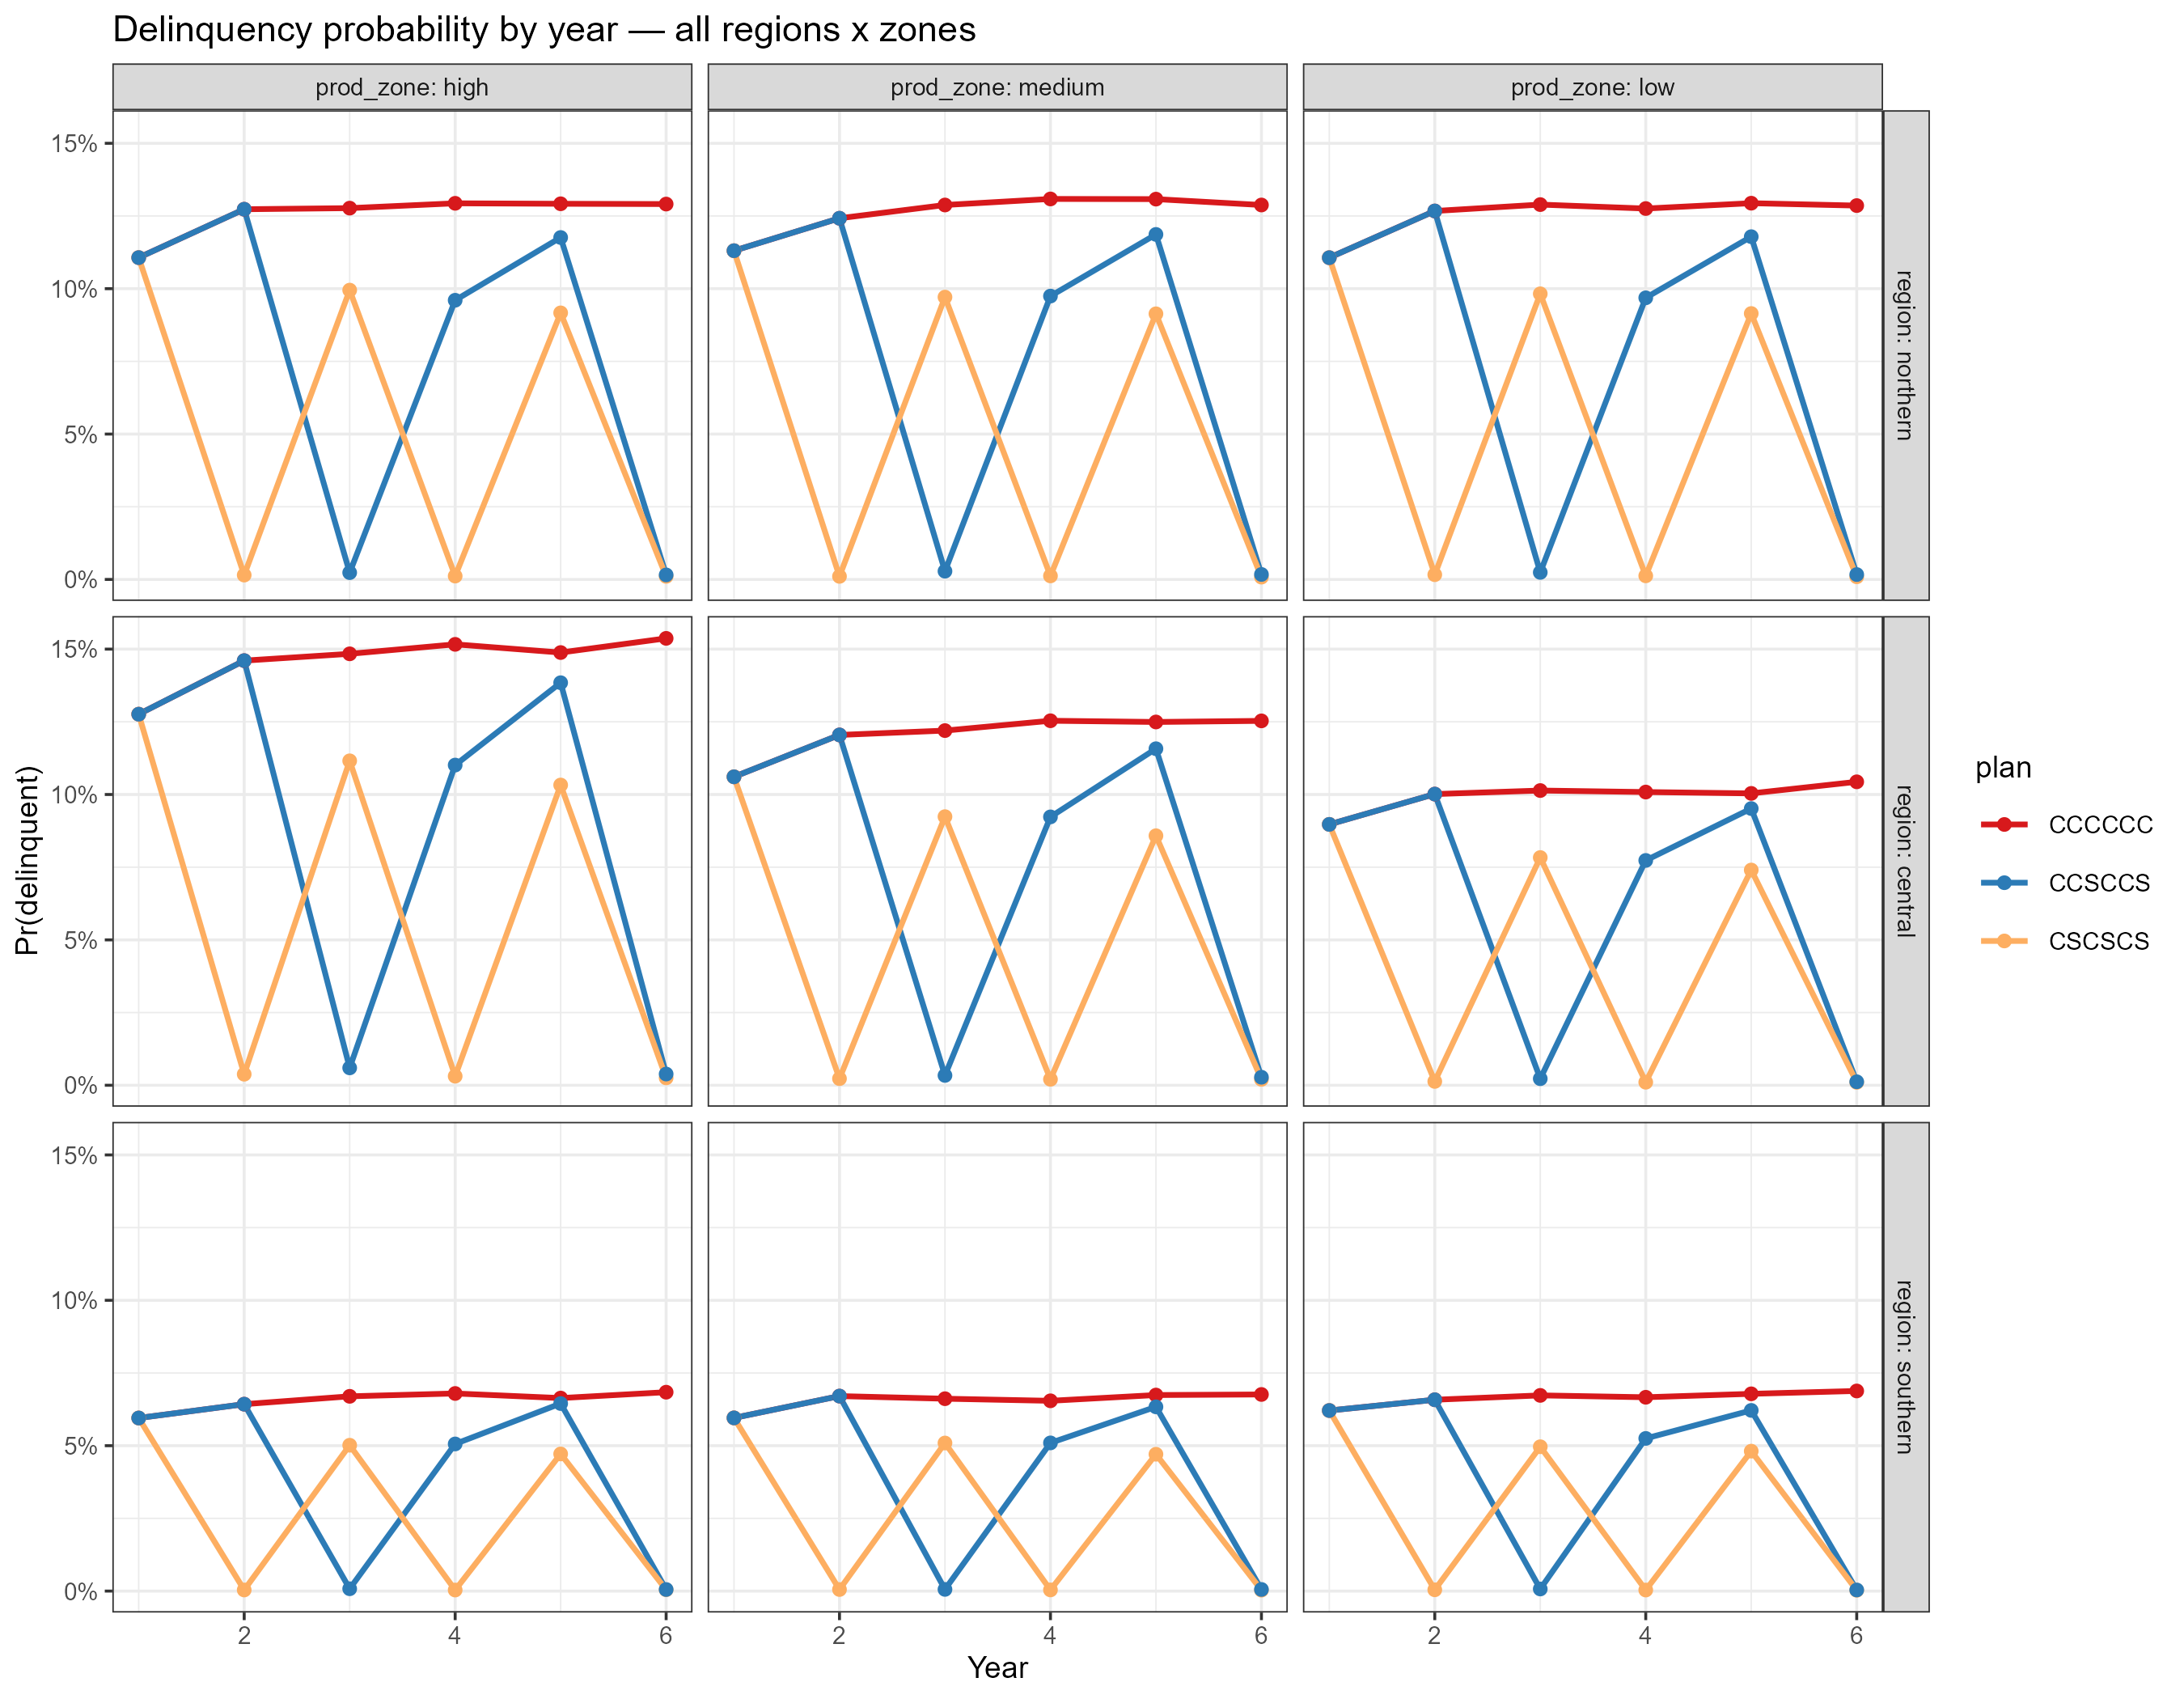
\includegraphics[width=16cm]{figs/fig_p_year_all.png}
    \caption{Soy years reset the debt cycle - the sawtooth}
    \label{fig:fig_p_year_all} 
\end{figure}

Continuous corn produces a flat hazard — roughly 12–15 percent per year, with a mild upward drift as debt accumulates. There is no good year, no recovery, just a steady grind. The rotation plans are different in kind, not just in level. They produce a sawtooth: the hazard collapses to near zero in soybean-harvest years and rebuilds during corn years. Under strict alternation, the flat segments fall on years 2, 4, and 6. Under 2-corn / 1-soy, they fall on years 3 and 6.

The mechanism is the debt reset. Soybean production costs roughly 70 percent of corn in the FBFM data, so a soybean year originates on a smaller spring loan, which makes the harvest-time obligation easier to clear even in a mediocre revenue year. When the soybean harvest retires the accumulated rollover balance from prior corn years, the farm enters the next corn run with near-zero carried debt — starting the cycle over. The six-year cumulative probability is not a smoothed average of annual risks. It is the result of intermittent arrests in a compounding process.

This matters for how we read the agronomic literature. \cite{Bullock1992} and \cite{Seifert2017} show that rotation raises corn yields; the financial benefit here is partly independent of that. Even when corn yield distributions are held identical across plans — removing the yield-benefit channel entirely — rotation still cuts delinquency, because the soybean year is a debt reset regardless of what it does to subsequent corn yields. Agronomic and financial channels stack.

\begin{figure}[H]
    \centering
    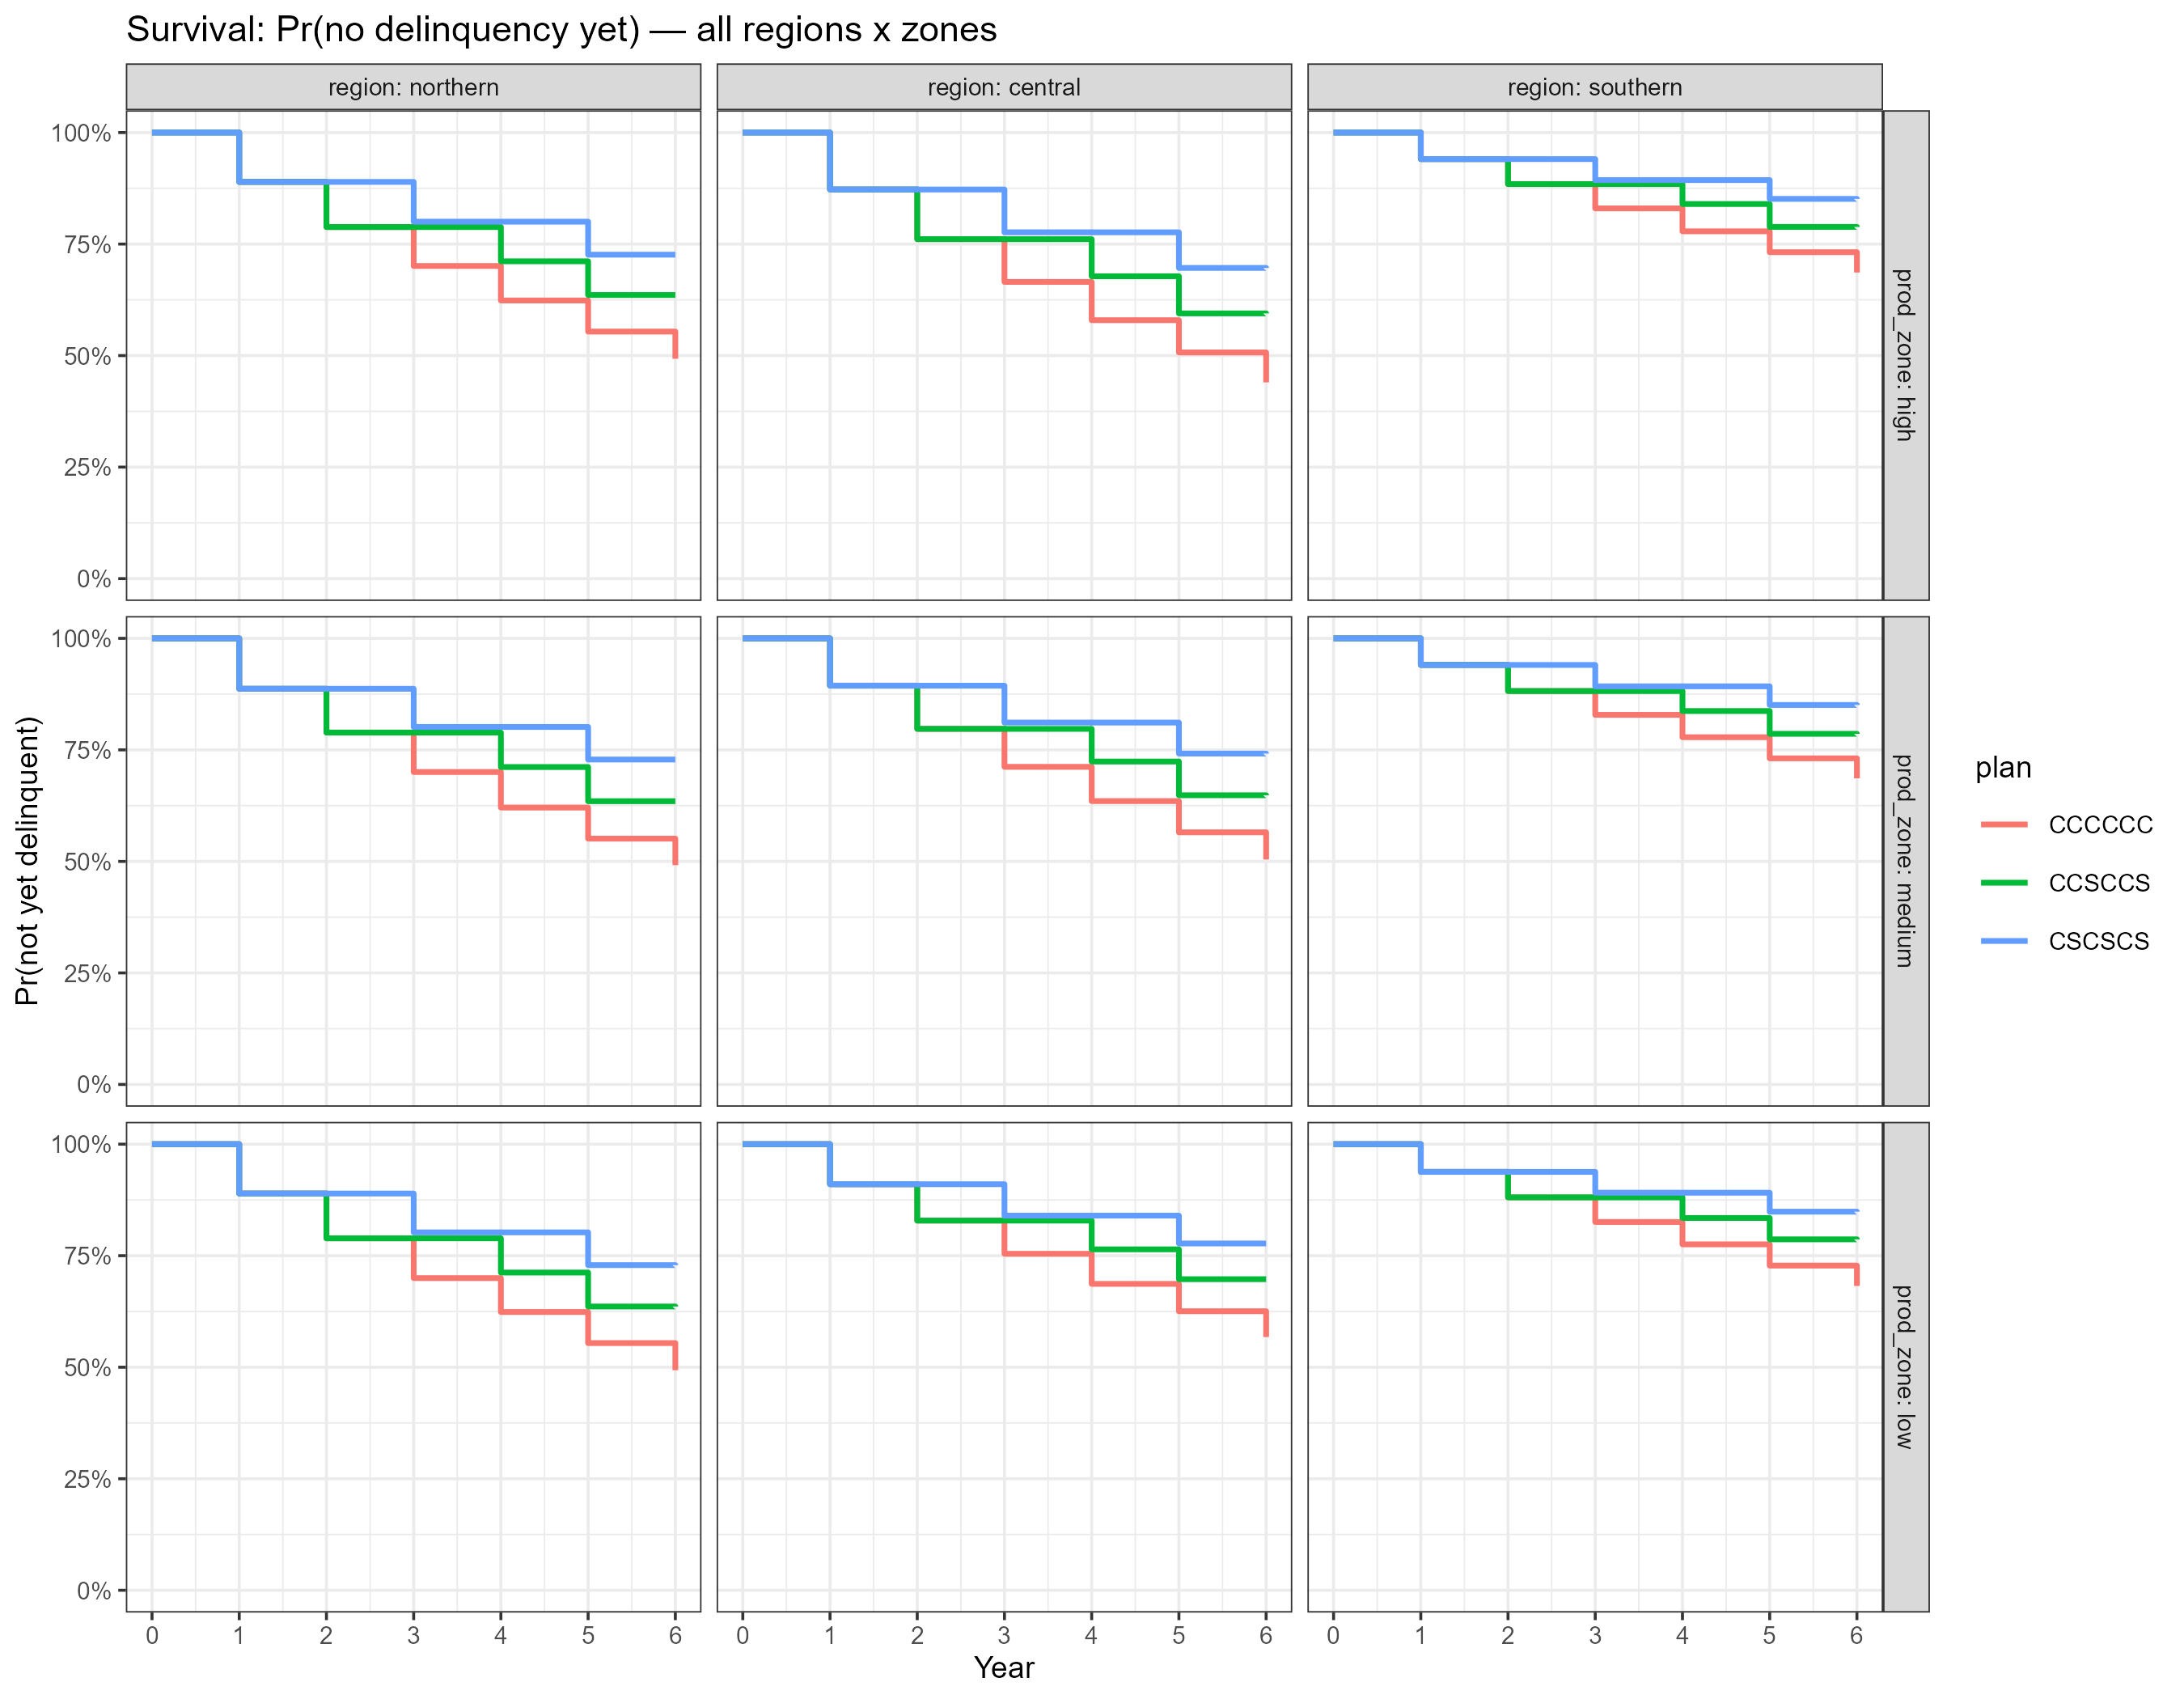
\includegraphics[width=16cm]{figs/fig_p_surv_all.png}
    \caption{Survival curves show where rotation pulls farms apart}
    \label{fig:fig_p_surv_all} 
\end{figure}

Figure \ref{fig:fig_p_surv_all} reports the corresponding survival curves, the probability that a field has \textit{not yet} experienced a delinquency event by year $t$. The step structure mirrors the sawtooth: drops in survival concentrate in corn years, flat segments occupy soybean years. By year 3, the survival gap between continuous corn and strict alternation has widened to 15–20 percentage points; by year 6, alternation preserves 70–85 percent of fields in solvency across regions and zones, while continuous corn retains only 45–70 percent. The earliest delinquency events, therefore, do most of the lasting damage, since once a field enters the delinquency state under continuous corn, it tends not to leave it.

\subsection{\label{subsec:peak_demand}Peak operating-loan demand}

\begin{figure}[H]
    \centering
    \includegraphics[width=16cm]{figs/fig_peak_loan_all.png}
    \caption{Peak loan demand stays under common credit limits}
    \label{fig:fig_peak_loan_all} 
\end{figure}

A related concern for lenders is not just whether a borrower becomes delinquent, but whether the demanded operating loan exceeds a credit ceiling the lender is willing to extend. Figure \ref{fig:fig_peak_loan_all} reports the distribution of peak gross spring loan demand ($L_t = C_t + B_{t-1}$) over the six-year horizon, with representative credit ceilings of $\$700$, $\$900$, and $\$1{,}200$ per acre overlaid.

In every cell, the median peak loan clusters between $\$500$ and $\$550$ per acre, well below any of the three ceiling values. Rationing is therefore rare under all three plans at any calibrated limit. The rotation effect on the \textit{distribution} of peak demand is nonetheless economically meaningful: continuous corn produces a right tail that approaches $\$700$ in the high-pressure cells, while strict alternation truncates the distribution roughly $\$50$ per acre lower. The safety margin between expected demand and the binding ceiling is therefore $\$50$ per acre wider under rotation.

This finding is consistent with a standard interpretation: rotation lowers not only the \textit{probability} of delinquency but also the \textit{exposure} a lender faces conditional on observing the borrower. A lender using rotation history as a credit-risk factor (Section \ref{sec:implications}) would price rotation borrowers' risk lower both because they default less and because their peak demand is farther from the lender's exposure limit.

\subsection{\label{subsec:natural_hedge}The natural hedge: rotation and correlation are partial substitutes}

Figure \ref{fig:fig_p_debt_all} isolates the natural-hedge effect by reporting the mean year-end carried debt under two specifications: the baseline correlated simulation (price and yield drawn from the joint copula, "hedge active") and a counterfactual independent simulation (price and yield drawn from the marginals as if uncorrelated, "no hedge"). The vertical gap between the two specifications is the natural hedge benefit.

\begin{figure}[H]
    \centering
    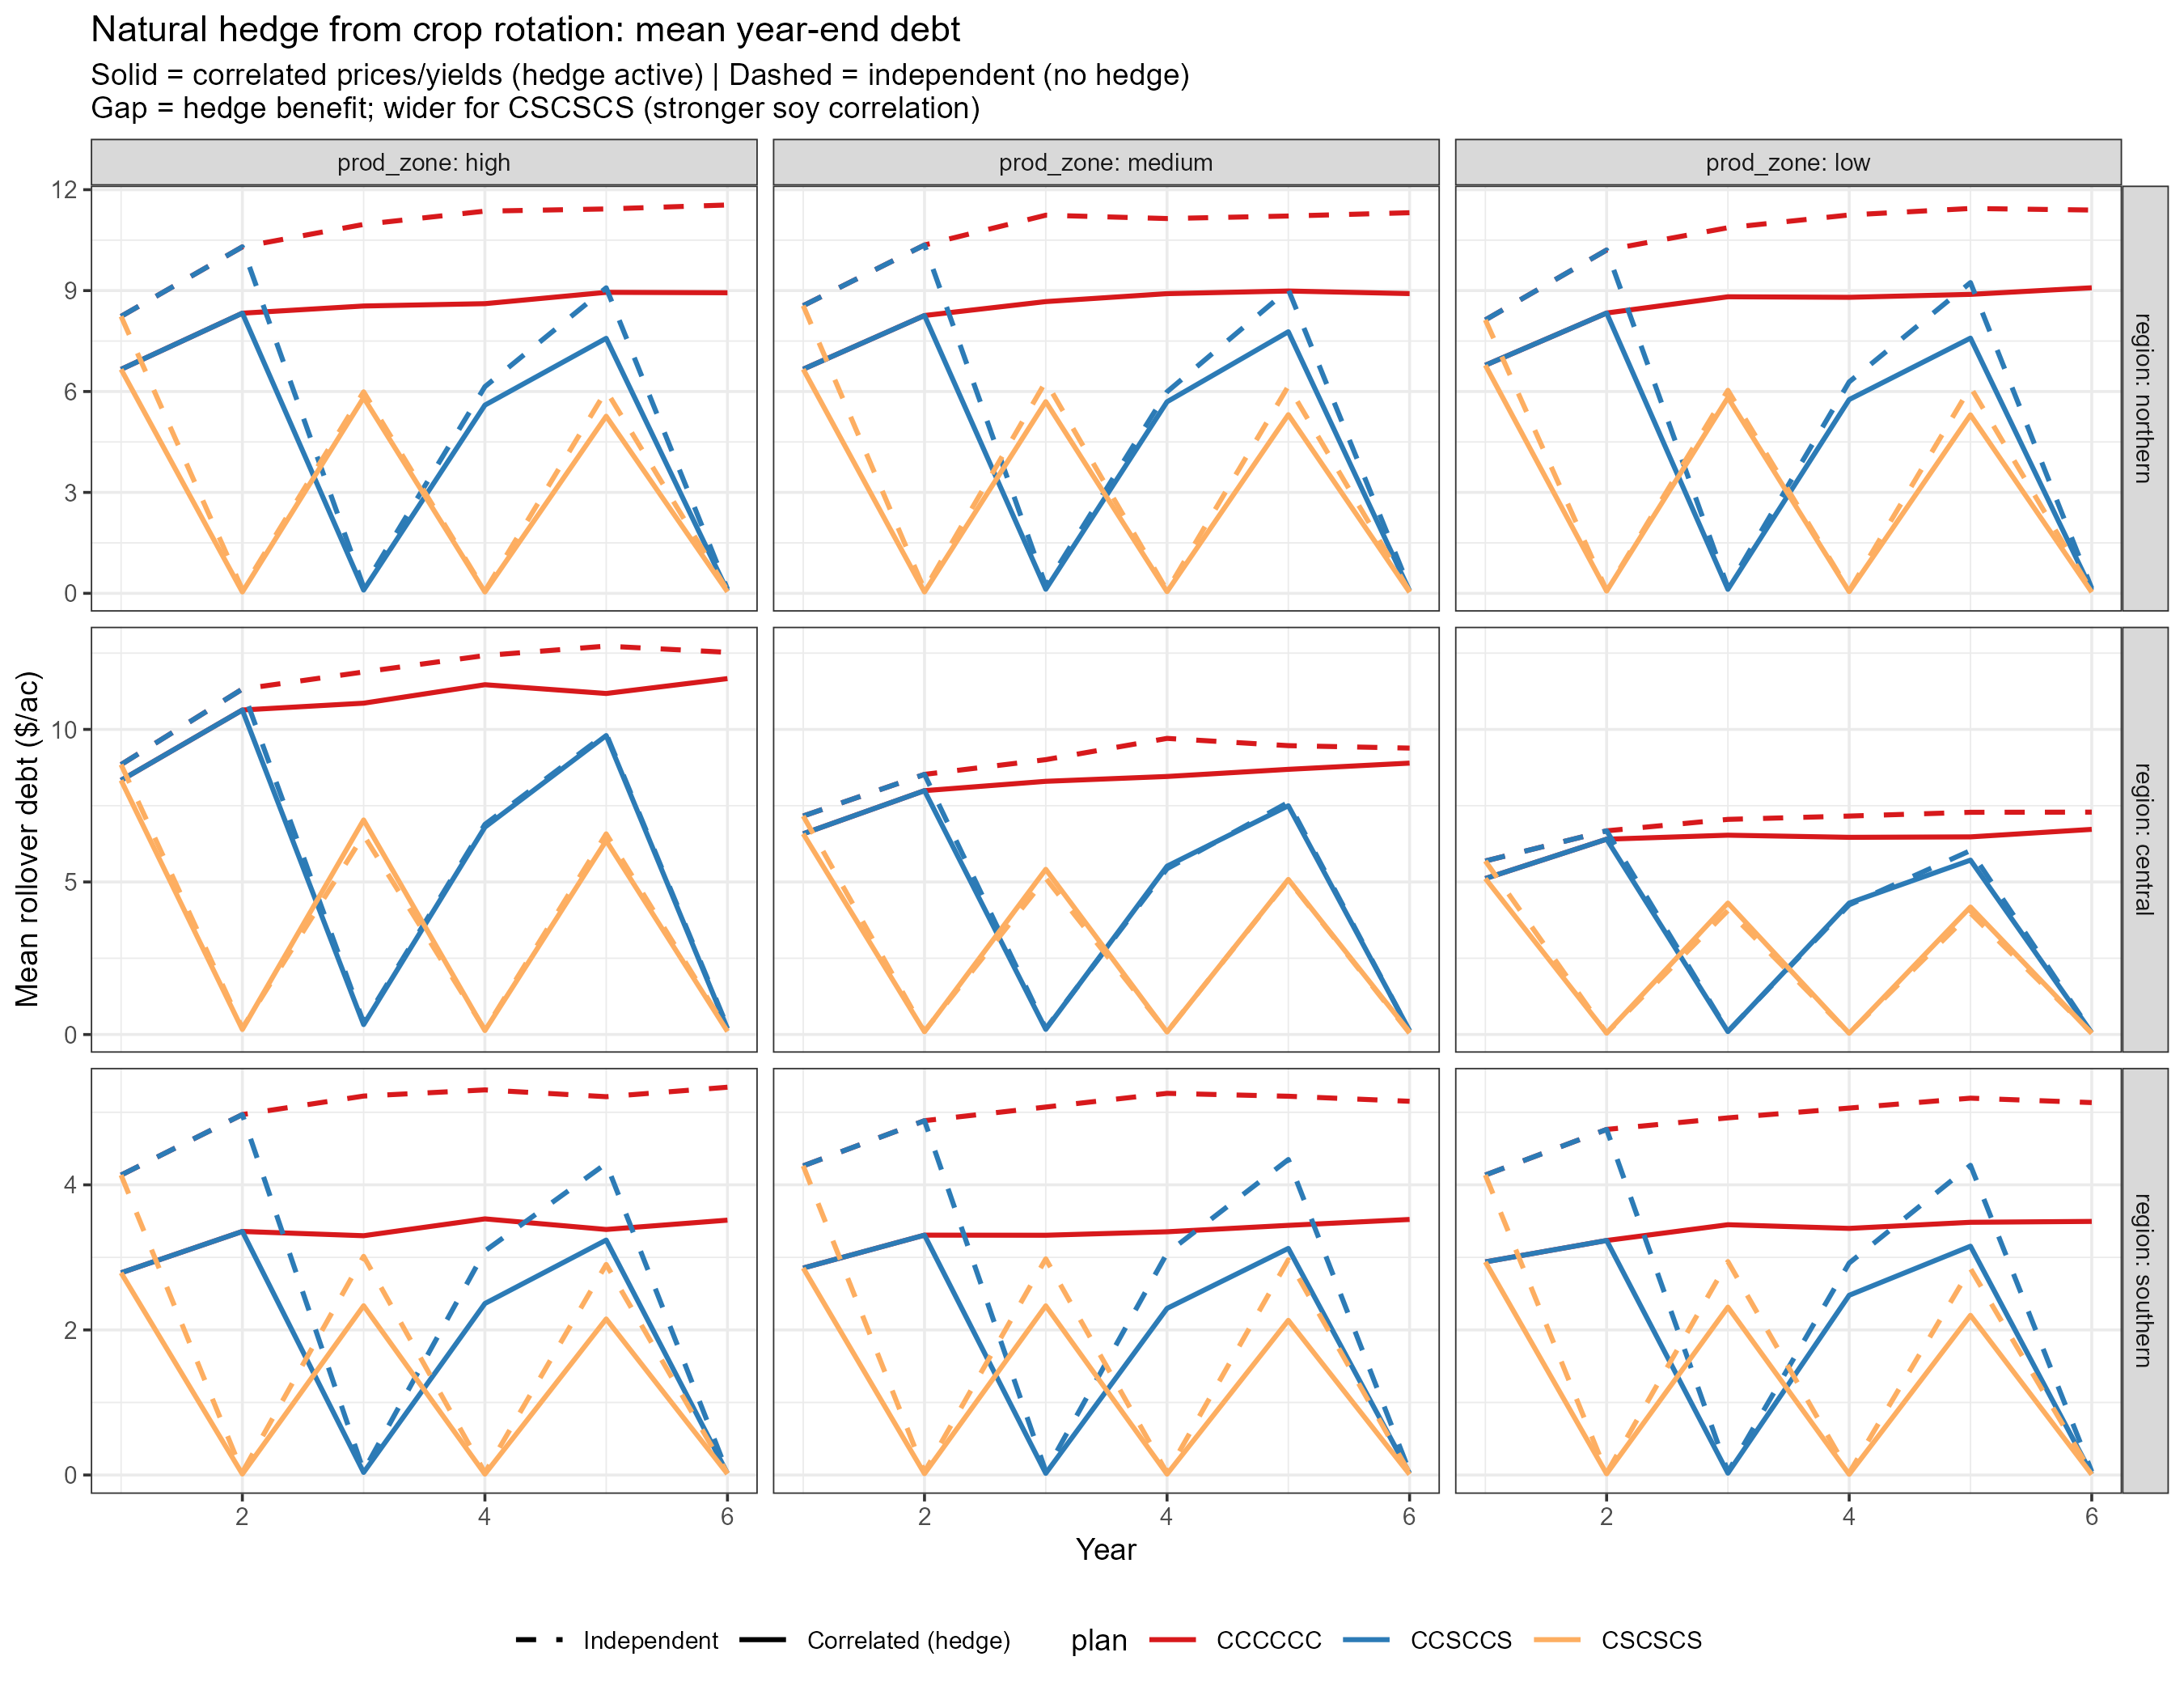
\includegraphics[width=16cm]{figs/fig_p_debt_all.png}
    \caption{The natural hedge mostly helps continuous corn}
    \label{fig:fig_p_debt_all} 
\end{figure}

The result is striking: the hedge gap is widest for continuous corn (red), where it averages 1–2 dollars per acre of year-end debt, and narrows to essentially zero for the two rotation plans. Rotation and the natural hedge are therefore \textbf{partial substitutes} in the cash-flow space, not complements. Continuous corn benefits from the hedge because it has nothing else to arrest the debt-rollover process: a high national yield depresses price and a low national yield raises it, partially offsetting the revenue shortfall that would otherwise compound into rollover debt. Rotation plans benefit less because they have already accomplished what the hedge would otherwise do: periodically driving carried debt to zero in soybean years, leaving the hedge with little remaining buffering work to perform.

This substitutability is a contribution of the multi-year framing. In a one-year revenue-protection setting, the natural hedge is unambiguously beneficial and additive to whatever other risk management the farmer employs. In the multi-year credit-risk setting, the hedge is most useful to the borrower with no other instrument (i.e., the continuous-corn borrower) and less useful to the borrower who rotates. The implication for the natural-hedge literature \citep{Finger2012, Ramsey2019} is that field-level hedge magnitudes estimated on single-year revenue data may \textbf{overstate} the hedge's marginal contribution to multi-year financial
resilience, because they do not net out the rotation channel that operates in parallel.

\subsection{\label{subsec:hedge_benefit}The hedge benefit in delinquency probability space}

Figure \ref{fig:fig_p_debt_all} establishes the substitutability result using the mean year-end carried debt. Figure \ref{fig:fig_p_bar_corr} translates the same comparison directly into the delinquency probability space, which is the paper's headline outcome and the most legible to lenders and insurers. For each of the nine region $\times$ zone cells, Figure \ref{fig:fig_p_bar_corr} plots the six-year delinquency probability under the independent specification (faded bar, no hedge) and the correlated specification (solid bar, hedge active), side by side for each rotation plan. The gap between the two bars within a plan is the hedge's marginal contribution to delinquency reduction, holding the rotation plan fixed.

\begin{figure}[H]
    \centering
    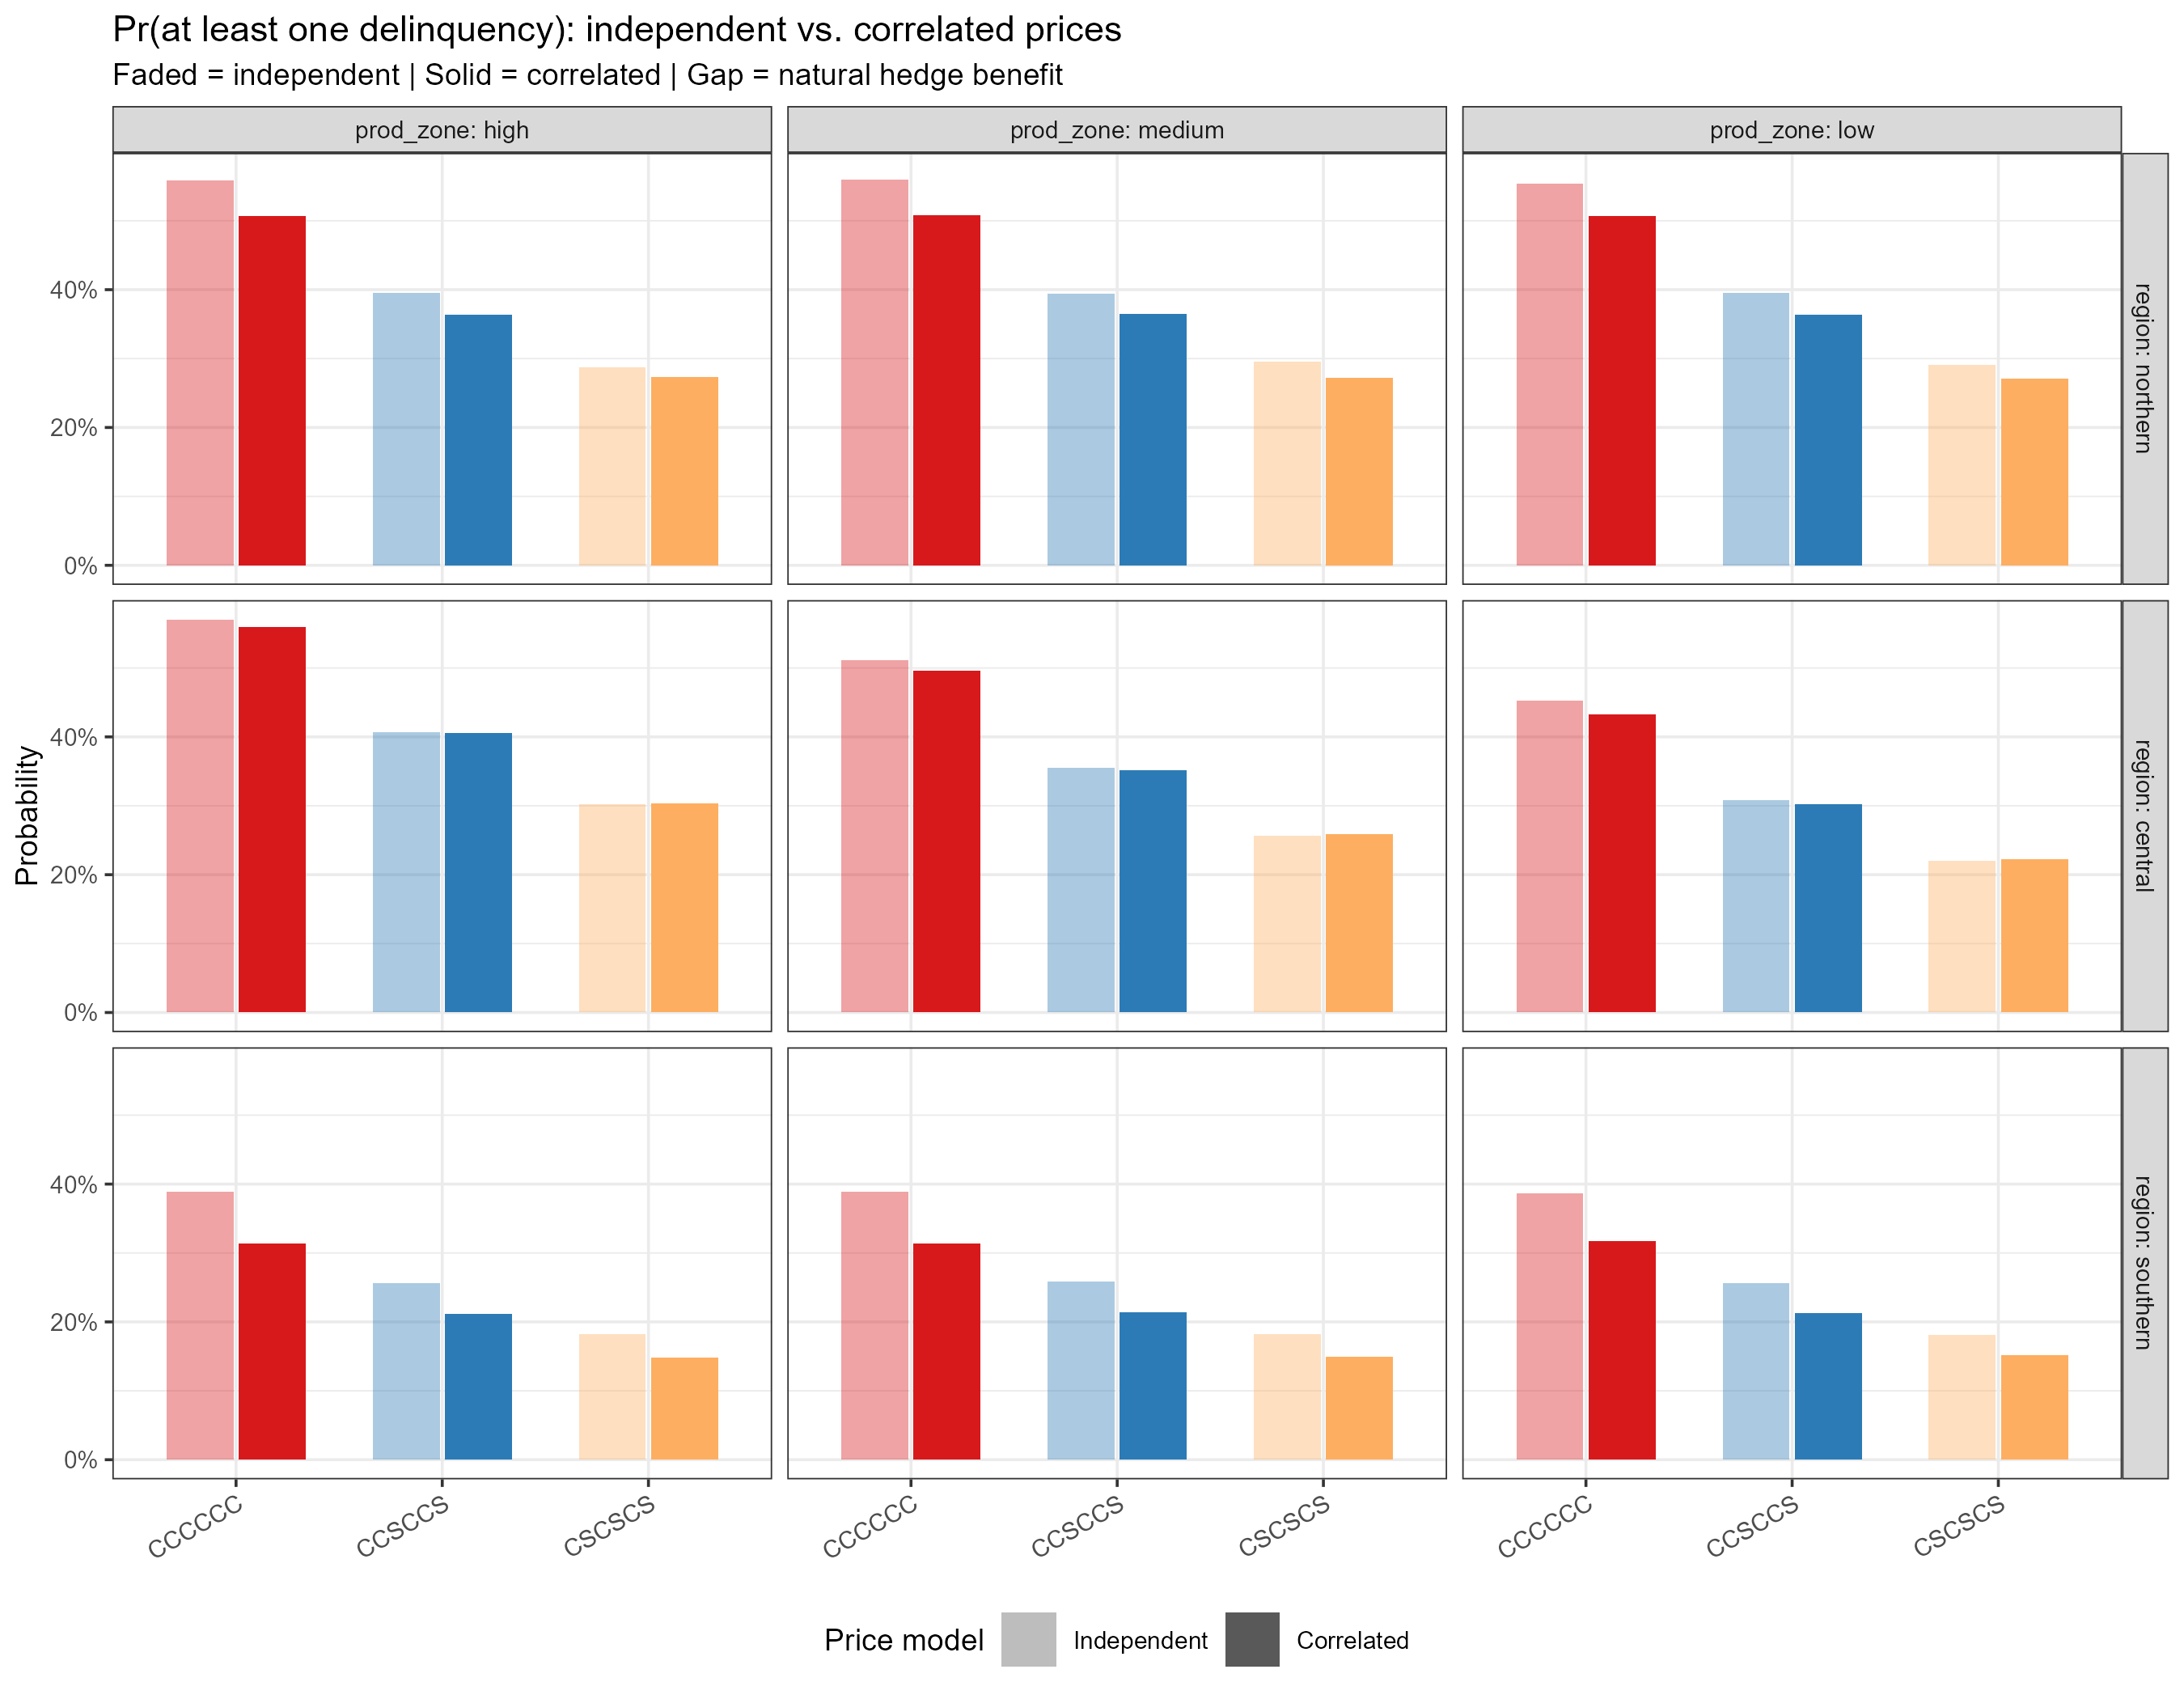
\includegraphics[width=16cm]{figs/fig_p_bar_corr.png}
    \caption{Price-yield correlation dampens the effects of rotations}
    \label{fig:fig_p_bar_corr} 
\end{figure}

Three features of Figure \ref{fig:fig_p_bar_corr} warrant emphasis.

\textbf{First, the hedge benefit is positive but uniformly small}. In every cell and every rotation plan, the solid bar is shorter than the faded bar, the negative price–yield correlation always reduces delinquency relative to the independent case. But the gap is narrow. In the northern and central rows, the hedge reduces the continuous-corn delinquency probability by approximately 2–4 percentage points; for the rotation plans, the reduction is 1–2 percentage points or less. Across the full 27-cell grid (nine region $\times$ zone cells $\times$ three rotation plans) the hedge never moves the needle by more than 4–5 percentage points. Against a baseline continuous-corn probability of 50–55 percent in the high-pressure cells, a 4-point reduction is economically modest.

\textbf{Second, the hedge benefit is largest for continuous corn and approximately zero for strict alternation}. This is the delinquency-space expression of the substitutability documented in Figure \ref{fig:fig_p_debt_all}. The faded-to-solid gap is visually largest for CCCCCC in every cell, and it narrows progressively across CCSCCS and CSCSCS, reaching near-zero for CSCSCS in most northern and central cells. The mechanism is the same: a rotation plan that resets carried debt in soybean years has already eliminated the rollover balance that the hedge would otherwise partially protect against. With no accumulated deficit to offset, the price–yield correlation is irrelevant.

\textbf{Third, the southern region is the partial exception}. In the south row, the hedge gap for continuous corn is visibly wider (roughly 7–9 percentage points) than in the north and central rows. Two features of the southern calibration explain this. Operating costs are lower, and the continuous-corn yield penalty is smaller in the south, so the baseline delinquency probability for CCCCCC sits around 31–32 percent rather than 50–55 percent. At this lower baseline, each percentage point of hedge benefit represents a larger \textit{relative} risk reduction, amplifying the visible gap. In addition, the debt-rollover chain under the southern continuous corn is less entrenched (carried balances are smaller in absolute terms) so the hedge has more proportional room to arrest the process before it crosses the delinquency threshold.

Taken together, Figures \ref{fig:fig_p_debt_all} and \ref{fig:fig_p_bar_corr} make the same argument from two angles. Figure \ref{fig:fig_p_debt_all} shows that the hedge reduces the \textit{level} of year-end carried debt, with the largest reduction for continuous corn and the smallest for rotation plans. Figure \ref{fig:fig_p_bar_corr} shows that this debt reduction translates into a modest and asymmetrically distributed reduction in \textit{delinquency probability}, modest because price risk dominates revenue variance (Section \ref{subsec:var_decomp}) and the hedge can only offset the covariance term, and asymmetric because rotation preempts the rollover channel through which the hedge would otherwise operate. The two instruments are substitutes, and the rotation plan that benefits least from the hedge is the one that needs it least. 

\subsection{\label{subsec:stress_test}Yield-shock stress test: the hedge under a localized corn shortfall}

Sections \ref{subsec:natural_hedge} and \ref{subsec:hedge_benefit} characterize the hedge benefit averaged over the full joint distribution of price and yield realizations. Figure 7 isolates the hedge's role under a specific, economically interpretable shock: a -12 percent corn yield shortfall applied only in year 3, with all other years held at their unconditional means. The experiment is run separately under the correlated and independent price specifications, so the gap between the two rows within each panel is again the natural-hedge benefit, here conditional on a known shock rather than averaged across the full simulation. Because year 3 is a soybean year under the CCSCCS plan, CCSCCS serves as a null control throughout: a corn yield shock in a soybean year mechanically produces no delinquency response, providing a clean within-figure placebo.

\begin{figure}[H]
    \centering
    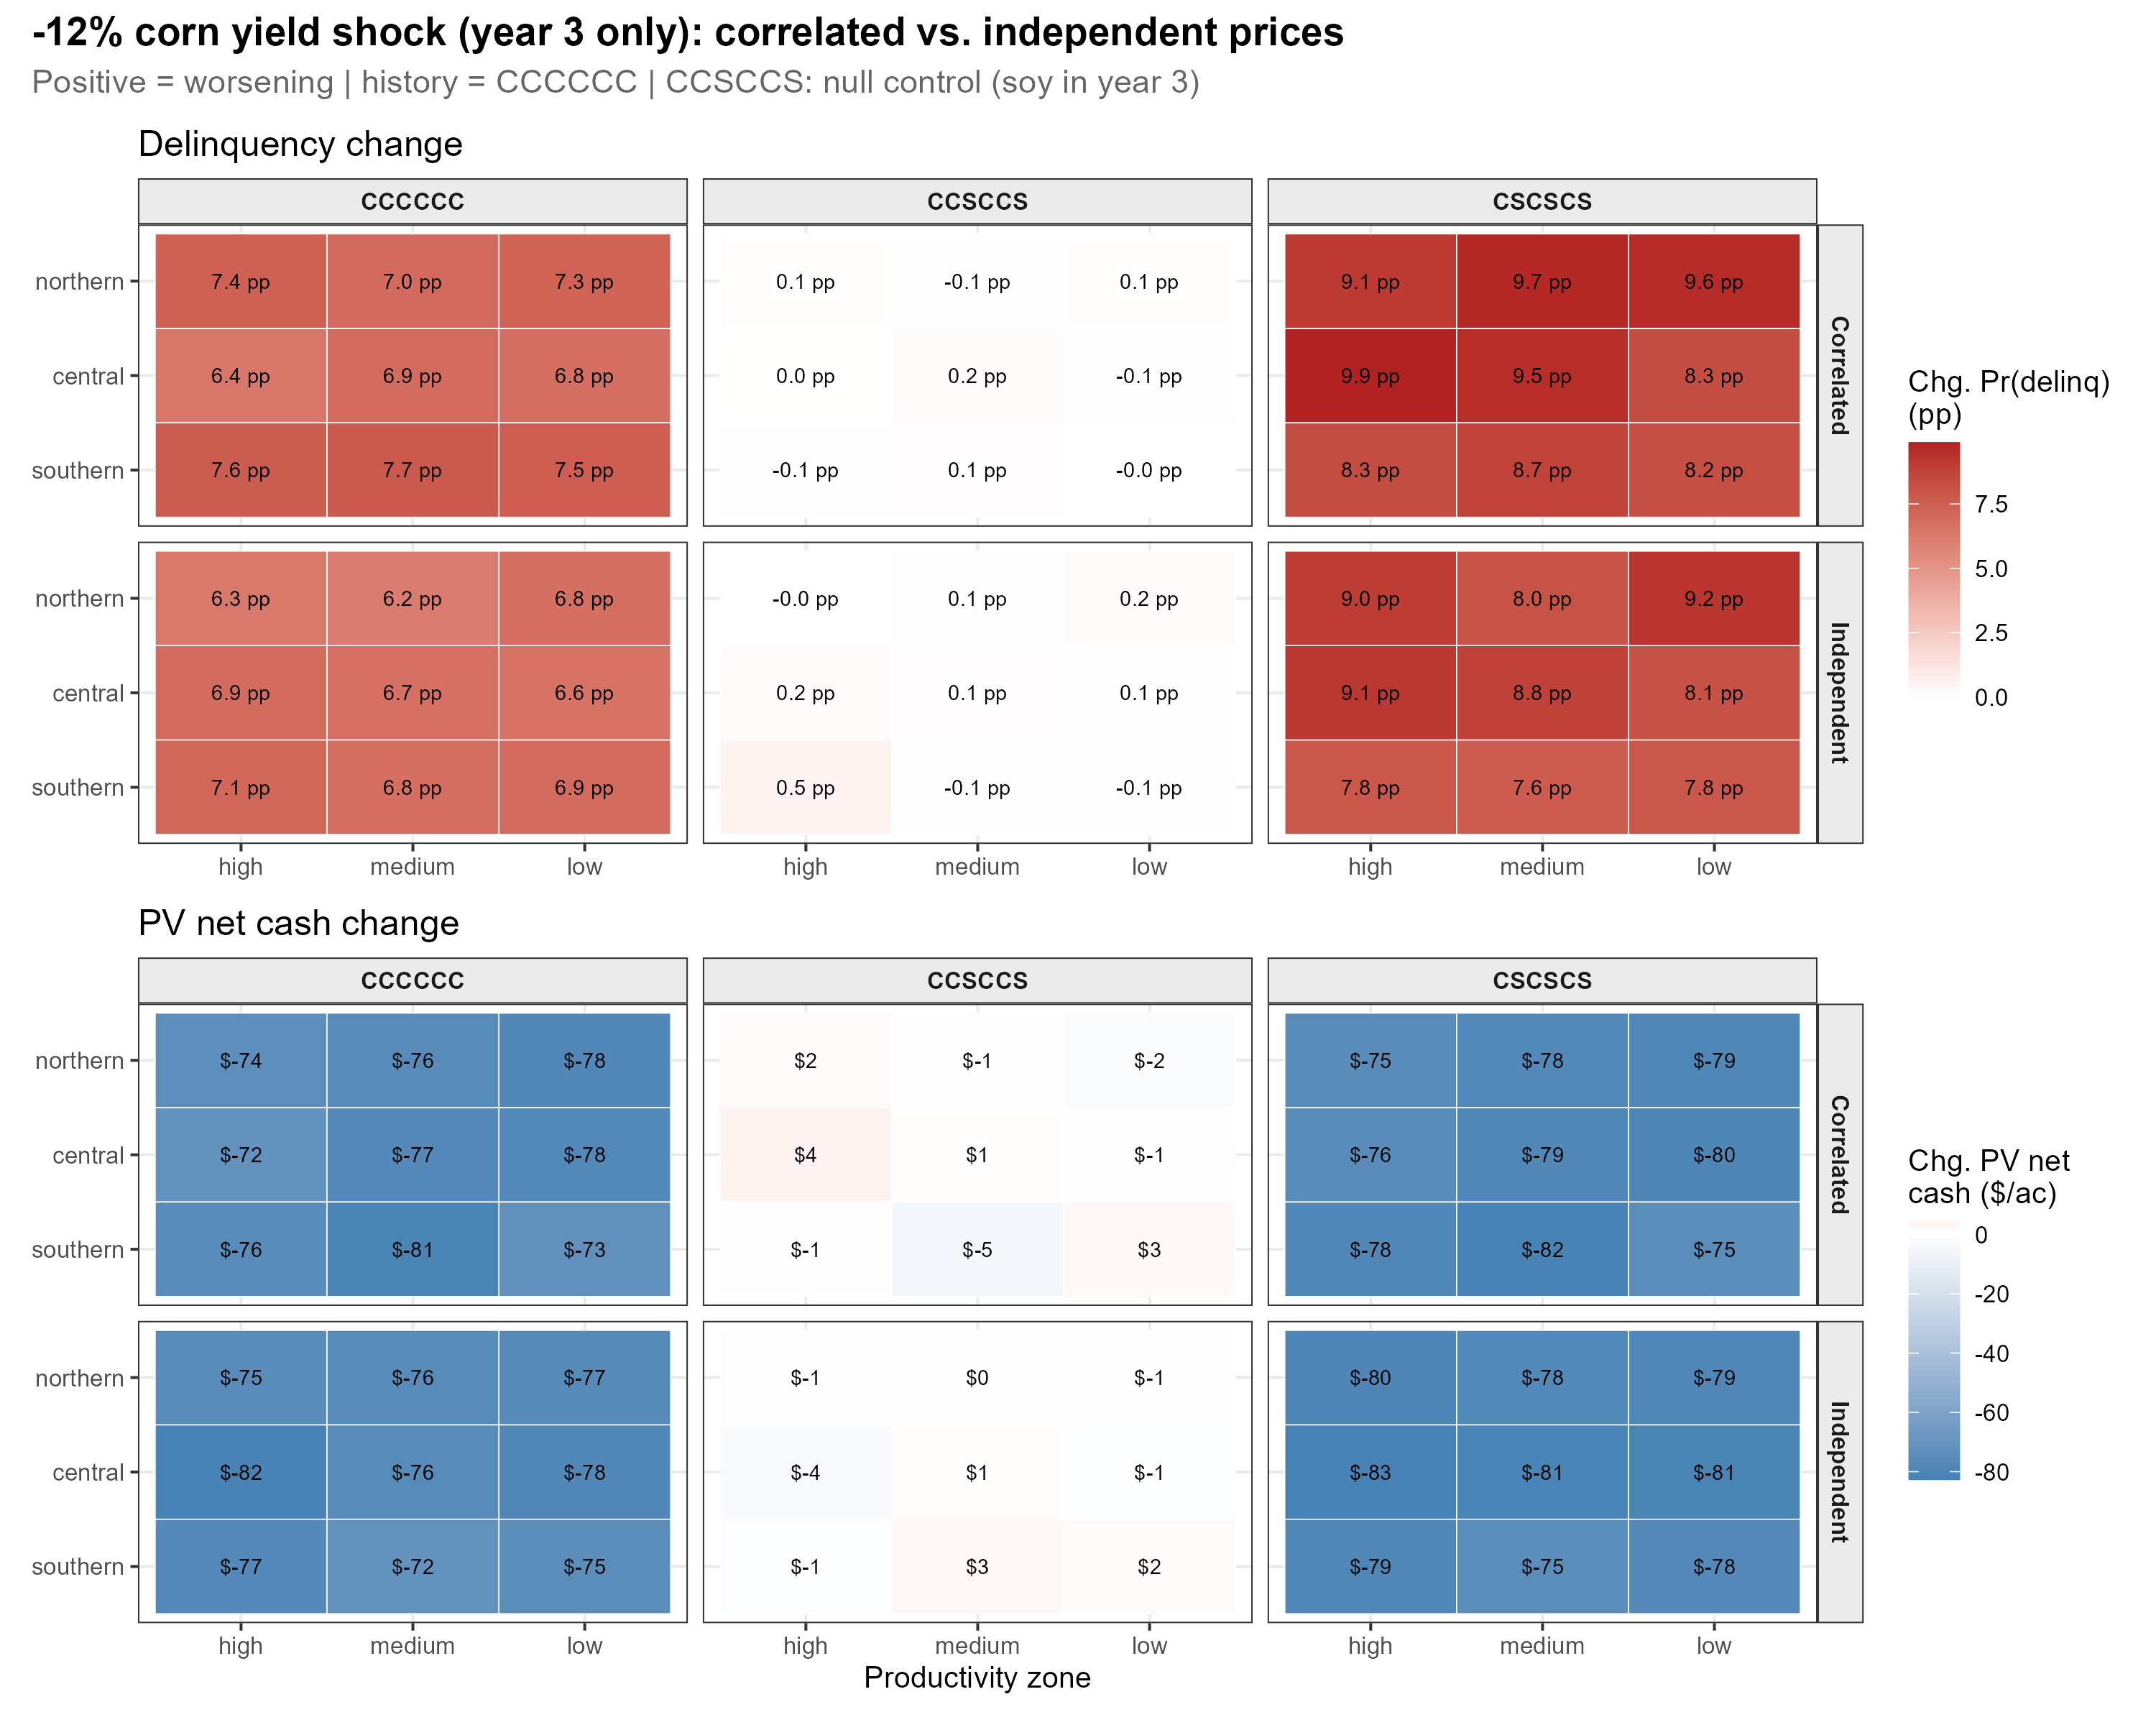
\includegraphics[width=16cm]{figs/fig_yield_compare_corr_vs_indep.png}
    \caption{Yield-shock stress test}
    \label{fig:fig_yield_compare_corr_vs_indep} 
\end{figure}

The figure has two panels. The top panel reports the change in six-year delinquency probability relative to the no-shock baseline (positive values indicate worsening). The bottom panel reports the change in present value of net cash flow over the six-year horizon (\$/acre; negative values indicate a loss). Both panels condition on a six-year history of CCCCCC for the CCCCCC plan and an analogous corn-heavy history for CSCSCS.

\textbf{The delinquency response is large for CCCCCC and CSCSCS, and zero for CCSCCS}. Under continuous corn, a single -12 percent yield shock in year 3 raises six-year delinquency probability by 6.4-7.7 percentage points across all region $\times$ zone cells under the correlated specification, and 6.2-7.1 percentage points under the independent specification. The correlated–independent gap here is small (roughly 0.3-0.7 percentage points), confirming that the hedge provides only modest additional protection against this type of shock, even when active. Under strict alternation (CSCSCS), year 3 is a corn year, so the shock hits; the delinquency response is even larger than under CCCCCC, ranging from 8.2 to 9.9 percentage points across cells. This is not counterintuitive: under strict alternation, year 3 is the first corn year after the initial year-2 soybean reset, so the field enters year 3 with near-zero carried debt (a favorable starting position), but a severe enough yield shortfall still generates a non-trivial probability of a first delinquency event, which the year-4 soybean year will then be in a position to arrest. The CCSCCS cells are uniformly near zero (-0.1 to +0.5 percentage points), as expected for a placebo applied in a soybean year.

\textbf{The PV cash response is symmetric across plans and specifications}. The bottom panel tells a different story: all three plans that plant corn in year 3 (CCCCCC and CSCSCS) show a cash loss of approximately \$72-\$83 per acre, and this figure is nearly identical across the correlated and independent rows. The hedge does not protect cash flow materially, it cannot, because the shock is a single-year idiosyncratic yield draw that does not move national supply enough to produce a meaningful price offset at the field level. The CCSCCS placebo shows near-zero cash changes of $\pm \$5$ per acre, consistent with no corn planted in year 3.

The asymmetry between the two panels is informative. The PV cash response is roughly equal across plans and price models: a -12 percent yield shock costs approximately the same dollar amount regardless of whether the plan is in rotation or hedge status. But the delinquency response differs substantially across plans, CSCSCS converts a yield shock of the same cash magnitude into a larger delinquency spike because it has not yet accumulated rollover debt going into year 3, meaning the shock must be absorbed entirely within that year rather than being spread across a pre-existing debt stock. This illustrates why delinquency probability and cash-flow loss are not the same object: the path the debt takes through the credit recursion matters, not just the terminal net present value. Rotation's debt-reset mechanism produces fields that are simultaneously more financially resilient on average (lower six-year delinquency, as documented in Section \ref{subsec:delinq_prob}) and more sensitive to a point shock in a corn year, because they carry less buffering debt into that year. A lender underwriting a rotation borrower therefore faces a different shape of credit risk, lower persistent default probability but a sharper single-year spike, than the continuous-corn borrower's flatter, more slowly compounding hazard. 

\section{\label{sec:robustness}Decompositions and robustness}
Section \ref{sec:results} establishes that rotation cuts delinquency and that the natural hedge is a modest substitute. Section \ref{sec:robustness} asks the deeper question of \textbf{what source of uncertainty} drives the residual risk that rotation does not eliminate. The variance decomposition (Section \ref{subsec:var_decomp}) attributes gross revenue variance to price and yield components. The Shapley decomposition (Section \ref{subsec:shapley}) attributes \textbf{delinquency probability} to the same two sources, using the cooperative-game fair-share framework. The two decompositions answer different questions and together pin down why the hedge is modest: price uncertainty dominates both variance and the causation of delinquency, leaving the hedge, which can only offset the price–yield interaction, with limited scope to operate. 

\subsection{\label{subsec:var_decomp}Variance decomposition}
For each plan-region-zone cell, we decompose the variance of annual gross revenue $R = P Y$ into the share attributable to price-only variation ($\text{Var}(P) \cdot E[Y]^2$ as a share of total gross variance) and the share attributable to yield-only variation ($\text{Var}(Y) \cdot E[P]^2$ as a share of total gross variance). The remainder, the covariance term $2 E[P] E[Y] \text{Cov}(P, Y)$, is negative under the calibrated copula and is reported separately as the hedge magnitude rather than being absorbed into either share.

\begin{figure}[H]
    \centering
    \includegraphics[width=16cm]{figs/fig_revenue_variance_decomp.png}
    \caption{Price dominates revenue variance}
    \label{fig:fig_revenue_variance_decomp} 
\end{figure}

Figure \ref{fig:fig_revenue_variance_decomp} reports the result. The price share is 86–89 percent of the gross variance across all plans, regions, and zones; the yield share is 11–14 percent. The split is remarkably stable across the simulation grid: rotation plans do not measurably change the \textit{composition} of revenue risk, only its level. The result is not a model artifact of the lognormal price assumption: the empirical price variance over 2008–2022 dominates the empirical yield variance for Illinois corn and soybeans by approximately the same ratio, and the copula merely inherits this asymmetry.

The implication is that the natural price–yield hedge can only do so much at the field level. Even if price and yield were perfectly negatively correlated, the hedge would offset only the price–yield covariance, at most a few percentage points of total variance, leaving the dominant price-driven variance intact. Rotation, which operates through the within-year debt timing rather than through revenue smoothing, sidesteps this limitation entirely.

\subsection{\label{subsec:shapley}Shapley decomposition of delinquency probability}

The variance decomposition speaks to how revenue varies, but delinquency is a threshold-crossing event, not a measure of variance. A 50-50 variance split between price and yield is fully consistent with a 99-1 split in \textbf{default causation} if the price shocks happen to live in the tail of the distribution that triggers rollover while yield shocks do not. To decompose the probability of delinquency directly, we follow the \cite{Shapley1953} cooperative-game value applied to risk-decomposition problems, as used by \cite{Shorrocks2013} and \cite{Israeli2007}.

Let $V(\mathcal{A})$ denote the delinquency probability when sources in $\mathcal{A} \subseteq \{P, Y\}$ are stochastic, and sources outside $\mathcal{A}$ are fixed at their unconditional means. The Shapley value for source $s$ is the average marginal contribution of $s$ to the delinquency probability across all orderings in which sources are added to the simulation. With two sources, the formula simplifies to:

\begin{equation}
    \phi_s = \tfrac{1}{2}\bigl[V(\{s\}) - V(\emptyset)\bigr]
       + \tfrac{1}{2}\bigl[V(\{P,Y\}) - V(\{P,Y\} \setminus \{s\})\bigr].
\end{equation}

The Shapley values are guaranteed to sum to $V(\{P,Y\}) - V(\emptyset)$, the total delinquency-causing variation, without an interaction residual.

\begin{figure}[H]
    \centering
    \includegraphics[width=16cm]{figs/fig_shapley_price_share.png}
    \caption{Shapley values}
    \label{fig:fig_shapley_price_share} 
\end{figure}

Figure \ref{fig:fig_shapley_price_share} reports the price share $\phi_P / (\phi_P + \phi_Y)$ across the plan-region-zone grid. The result is striking: the price share of delinquency causation ranges from 92 percent in the central-low cell under continuous corn to 100 percent in several southern-zone cells under strict alternation. Yield uncertainty contributes meaningfully to delinquency only in the central region under continuous corn, and even there, it accounts for less than one-tenth of the total.

The Shapley share is therefore \textbf{more lopsided} than the variance share (92–100 percent versus 86–89 percent). The reason is that yield shocks, while accounting for 11–14 percent of revenue variance, tend not to generate the tail revenue draws that trigger rollover. Yield distributions are bounded below by physical constraints (a zero-yield outcome is exceptional in the Illinois corn belt), while price distributions have longer left tails. Threshold-crossing events, therefore, disproportionately arise from price shocks, even relative to their already large share of revenue variance. The decomposition rationalizes Section \ref{subsec:natural_hedge}'s finding that the natural hedge is modest: the hedge can offset the small yield-driven component of delinquency, but the dominant price-driven component is unhedged by construction.

\subsection{\label{subsec:survival}Survival curves: when does the rotation effect materialize?}

The six-year cumulative delinquency probability reported in Section \ref{subsec:delinq_prob} is an integral across the horizon. Disaggregating it into a year-by-year survival function reveals \textit{when} the gap between rotation plans opens and which events do the lasting damage.

Figure \ref{fig:fig_p_surv_all} plots $\Pr[\text{no delinquency by year } t]$ for each plan across all nine regions $\times$ zone cells. Three patterns are immediate. First, the step structure of every curve mirrors the sawtooth in the per-year hazard: survival drops in corn years and holds flat in soybean years. Second, the gap between plans opens almost immediately. By year 3, the end of the first full corn-soy cycle, CSCSCS lies 15–20 percentage points above CCCCCC in every cell. The earliest delinquency events, which occur in the first corn run before any soybean reset has arrived, are therefore the events that matter most for the cumulative probability. Third, the separation is durable: the gap does not narrow in later years because continuous corn provides no debt-reset mechanism to recover from early delinquency.

The survival curves also document the limited recovery available under continuous corn. Once a field enters the delinquency state, i.e., once $B_t > 0$, the carried balance enlarges the following year's spring principal, raising the revenue threshold that must be cleared to return $B_{t+1}$ to zero. In the absence of a soybean year to break the chain, this threshold rises faster than the unconditional mean of revenue, so the conditional probability of a second consecutive delinquency exceeds the unconditional annual hazard of 12–15 percent. The result is that survival under continuous corn decays faster than a flat-hazard Kaplan–Meier curve would predict, whereas survival under rotation is approximately piecewise flat between resets. By year 6, strict alternation preserves 70–85 percent of fields in solvency across regions and zones; continuous corn retains only 45–70 percent.

The implication for lenders is practical. The 15–20 percentage-point survival gap materializes within the first loan-renewal cycle, not over a distant planning horizon. A lender observing a borrower's first two or three years of operating-loan history is already observing the consequence of the rotation choice: the borrower who has rotated arrives at year-3 renewal with a near-zero carried balance, while the continuous-corn borrower may be carrying a compounded deficit from one or more prior shortfalls. Rotation history observable in CDL imagery thus predicts not only the eventual six-year default probability but also the early trajectory of the credit relationship.

A second robustness exercise reports the simulation under an alternative delinquency rule ("over-limit" rather than end-balance-positive), with the underlying cumulative cash-flow object shown in Figure \ref{fig:fig_p_cf_all}. The absolute delinquency levels fall, naturally, since a positive balance below the credit ceiling no longer counts, but the relative ranking of plans and the sawtooth pattern in per-year hazards both survive. Figure \ref{fig:fig_shapley_abs} in Appendix \ref{sec:appendix_B} reports the absolute Shapley values underlying the normalized shares in Figure \ref{fig:fig_shapley_price_share}, confirming that the price-driven component dominates not just relatively but also in absolute terms. 

\section{\label{sec:implications}Implications}
The simulation produces three results with direct implications for parties who price farm credit risk and design crop insurance.

For \textbf{lenders}, rotation history is an observable, verifiable risk factor that current underwriting does not price. Two farms with identical balance sheets but different six-year rotation states face six-year delinquency probabilities that differ by a factor of two or more in the simulation, 55 percent versus 30 percent in the central-high Illinois area, with comparable multiplicative differences in other cells. CDL-derived rotation histories are publicly available at the field level, requiring no additional borrower disclosure, and the conditioning effect on delinquency is robust across the simulation grid. A credit-scoring model that incorporates rotation alongside conventional balance-sheet measures would assign strictly different scores to the two otherwise identical farms, in a direction the simulation argues is correct.

For \textbf{insurers}, the multi-year delinquency object identified here is not what Revenue Protection (RP) products price. RP premiums are calibrated to the single-year loss-cost ratio, which approximates $E[\max(0, \text{guarantee} - \text{revenue})]$ based on a one-year distribution. The single-year object does not see the rollover channel that converts a year-1 shock into a multi-year default cascade. A corn-heavy producer with a high one-year revenue distribution and a poor multi-year survival distribution may therefore appear cheap to insure on the single-year metric and expensive on the multi-year metric. The pricing implication is that RP premiums calibrated on single-year loss ratios systematically understate the \textit{insurance value} of rotation, since rotation's largest financial benefit accrues specifically to the multi-year delinquency dimension that RP does not see. This is a contribution to the credit-insurance interaction literature \cite{Ifft2013, IfftKuethe2015, Lee2024}: the federal crop insurance program may be inducing greater use of debt precisely because the rate structure does not reward the rotation choice that would reduce multi-year ruin.

For \textbf{extension and policy}, the financial case for rotation now parallels the agronomic and soil-health cases. Rotation's documented benefits for soil organic carbon, nitrogen-use efficiency, and pest pressure \citep{Bullock1992} are matched here by a balance-sheet benefit that is independent of the agronomic channel and additive to it. The financial argument is concrete and quantifiable in a way that the agronomic argument is not always: a 25-percentage-point reduction in six-year delinquency probability is an immediately legible benefit to the producer, regardless of whether the producer values the soil-health benefits. This complementarity strengthens the case for conservation programs that promote rotation, cover crops, and reduced tillage. It also matters in light of the empirical adoption pattern. \cite{socolar2021} documents that the U.S. Midwest rotation diversity has been declining for a century, with simplification concentrated on the most productive land and reinforced by proximity to biofuel plants and grain elevators, i.e., by policy-driven infrastructure that raises the relative return to corn. The agronomic argument has not been sufficient to halt this trend. A financial argument visible to lenders and insurers, the parties who actually price farm credit risk, is a candidate countervailing lever, operating not through producer education but through the price of credit itself.

We do not interpret these results as supporting an immediate mandate for rotation as a precondition for access to federal credit or insurance. The simulation imposes no individual heterogeneity in risk preferences or production technology, and the rotation effect averages over fields that might rationally choose continuous corn for reasons the simulation does not capture (off-farm income, livestock integration, non-standard cost structures). The case for incorporating rotation into underwriting is therefore one of \textit{risk-pricing accuracy}, not of behavioral mandate: a lender or insurer who prices a continuous-corn borrower at the same risk premium as an otherwise-identical rotation borrower is mispricing risk, regardless of whether continuous corn is the right choice for either farmer.

\section{\label{sec:conclusion}Conclusion}
This paper develops a simulation framework that combines rotation-conditioned yield distributions with an explicit operating-credit cash-flow recursion to produce multi-year delinquency probabilities for Illinois corn-belt farms. The framework's combination is, to my knowledge, new: the rotation-yield literature stops at yield, the dynamic-crop-choice literature stops at the optimal policy, and the farm-credit-risk literature treats yield as a single aggregate input. The combination delivers an empirical object, the rotation-conditional six-year delinquency probability, that current credit and insurance models do not produce.

Several findings emerge. First, rotation reduces six-year delinquency probability by approximately 25 percentage points relative to continuous corn in high-pressure cells, with the reduction concentrated in soybean-harvest years through a debt-reset mechanism. The per-year hazard exhibits a sawtooth pattern that distinguishes the mechanism from any uniform risk-smoothing explanation. Second, price uncertainty dominates both revenue variance (86–89 percent) and delinquency causation (92–100 percent), leaving the natural price–yield hedge with limited scope to operate. The hedge is most useful for the continuous-corn borrower who has no other risk-management instrument and is essentially redundant for the rotation borrower. Third, a year-2 soybean price placebo confirms that the rotation effect operates through the timing of soybean revenue relative to rollover debt, not through any aggregate price channel.

The findings imply that rotation history is a missing variable in the credit-risk and crop-insurance models used by lenders, insurers, and regulators. The variable is observable and verifiable in publicly available CDL imagery, and the simulation indicates that incorporating it would materially improve the accuracy of risk pricing. The case is strongest for multi-year insurance products that price ruin rather than single-year shortfall; the simulation suggests these products would price rotation as a strictly favorable feature of the covered farm.

Three extensions are natural. First, the simulation holds the rotation policy fixed; an extension that endogenizes the rotation choice, under a credit-risk-sensitive farmer who internalizes the multi-year delinquency probability, would speak to the equilibrium response of rotation choice to a hypothetical credit-pricing reform. Second, the delinquency object is binary in the current framework; a loss-given-default extension would convert the probability into a dollar-denominated expected loss that maps directly into pricing. Third, the framework is built on Illinois corn-belt data, where the two crops in rotation share infrastructure, equipment, and markets; extending to a region with more heterogeneous crop options (e.g., the southeastern U.S. cotton-peanut-soybean rotation) would test whether the debt-reset mechanism generalizes beyond the corn-soybean case.

The deeper contribution of the paper is methodological: that financial outcomes for farms are path-dependent in a way that current models do not capture, that the path dependence is rotation-conditional in a way that current credit-risk models do not see, and that the resulting mispricing has direct implications for an industry, agricultural lending and insurance, that intermediates approximately $\$220$ billion of non-real-estate farm debt in the United States, of which operating loans form a substantial share \citep{usda2026}. The framework is one attempt to close that gap; the rotation-as-credit-risk-factor framing is, we hope, the beginning of a broader conversation.

\appendix
\section{\label{sec:appendix_A}Appendix A: Calibration values and computational details}
\subsection{\label{subsec:parameter_values}Baseline parameter values}
Table \ref{tab:baseline_pars} reports the baseline values of every parameter that enters the simulation. Values not directly identifiable from the panel are calibrated from independent industry sources, with the source noted in the third column.

\begin{table}[!ht]
    \centering
    \begin{tabular}{lll}
    \hline\\
    \textbf{Parameter} & \textbf{Baseline value} & \textbf{Source}\\
    \hline\\
Operating-loan rate $i$ & 9.0\% APR & Federal Reserve Bank of Chicago\\
 & &  AgLetter, sample-period midpoint\\
 \\
Accrual window & 9 months & Convention for Illinois corn belt\\
& (March planting $\rightarrow$ October harvest) & \\
\\
Initial carried debt $B_0$ & \$0 / acre & Steady-state simplification\\
\\
Corn operating cost $C^{c}$ & Crop-specific Farmdoc cost-of-production & University of Illinois - Farmdoc\\
\\
Soybean operating cost $C^{s}$ & Crop-specific Farmdoc cost-of-production & University of Illinois - Farmdoc\\
\\
Aggregate price-yield & $-0.45$ & Estimated from national\\
correlation $\hat\rho$ & & NASS data, 2008–2022\\
\\\
Aggregate yield variance & $0.620$ & Field-panel variance\\
share $\sigma^2_{\text{agg}}/\sigma^2_Y$ & & decomposition\\
\\
Implied copula correlation $\rho^{*}$ & $-0.354$ & $\hat\rho \cdot \sqrt{0.62}$\\
\\
Price marginal & Lognormal, moment-matched & NASS Illinois cash prices\\
\\
Yield marginal & Empirical, conditional on $(s, c, z)$ & QDANN field panel\\
\\
Credit ceiling (low) & \$700 / acre & Sensitivity grid (see §3.3)\\
\\
Credit ceiling (mid) & \$900 / acre & Sensitivity grid (see §3.3)\\
\\
Credit ceiling (high) & \$1,200 / acre & Sensitivity grid (see §3.3) \\
\\
Delinquency rule & $B_t > 0$ (end-balance-positive) & Strictest definition\\
 & & alternative reported in §6.3\\
 \hline\\
    \end{tabular}
    \caption{Baseline parameter values}
    \label{tab:baseline_pars}
\end{table}

\newpage

\subsection{\label{sec:comp_details}Computational details}

Monte Carlo paths are drawn at $N = 50{,}000$ per (region $\times$ zone $\times$ plan $\times$ initial history) cell. Convergence is checked by partitioning the path set into two halves and confirming that the six-year delinquency probability agrees within 0.3 percentage points across halves in every cell. Cells with fewer than 30 panel observations for a given six-year history are pooled with the closest neighboring state (defined by Hamming distance on the crop sequence) to ensure sufficient empirical support for the conditional yield distribution.

\section{\label{sec:appendix_B}Appendix B: Robustness exercises}

Section \ref{sec:results} establishes the baseline results, and Sections \ref{subsec:var_decomp}–\ref{subsec:shapley} report the primary decomposition and robustness exercises. This appendix collects the secondary robustness exercises that are forward-referenced in the main text. Each exercise perturbs one calibration choice while holding the rest of the simulation fixed and reports whether the qualitative ranking of rotation plans and the central mechanism (the sawtooth) survive.

\subsection{\label{subsec:end_debt}Year-end debt distribution}
Figure \ref{fig:fig_p_debt_all} in the main text reports mean year-end carried debt under two price–yield dependence specifications (correlated and independent) to isolate the natural-hedge effect. Figure B.1 extends that object by adding the 75–90 percentile band around the mean debt trajectory under the baseline (correlated) specification, showing that rotation bounds the upper tail of carried debt, not just its mean.

The figure shows two features that an aggregate-only view would miss. First, the \textit{mean} debt path under continuous corn (red) is monotonically increasing in every cell, reaching \$9–12 per acre by year 6 in the high-pressure northern and central cells. The two rotation plans (green and blue) trace sawtooth paths that touch zero in soybean years and rebuild during corn years, with maxima below the continuous-corn level in every cell. Second, the 75–90 percentile band for continuous corn diverges from the band for rotations as the horizon lengthens, the upper tail of debt grows under continuous corn but is repeatedly truncated under rotation. The substantive point of Section \ref{sec:results} is therefore robust to a distributional view: rotation does not just lower mean debt; it bounds the upper tail, and the gap between plans is largest in the tail that matters for lender exposure.

\subsection{\label{subsec:param_fit}Parametric-fit robustness for the yield generator}
Section \ref{subsec:generator} estimates the rotation-conditional yield distribution $F_{Y \mid s, c, z}$ nonparametrically from the panel and notes that robustness to a parametric fit is reported here. The relevant question is whether the \textit{dispersion} of revenue at the rotation-plan level is preserved under a parametric (Beta or Gamma) alternative.

Figure \ref{fig:fig_revenue_cv} reports the coefficient of variation of \textbf{discounted six-year revenue} under the baseline nonparametric yield generator and the calibrated price copula. The CV ranges from 41\% in southern-zone rotation cells to 52\% in northern- and central-zone continuous-corn cells. Rotation cuts the CV by roughly 5 percentage points in every cell, a small but stable risk-reduction in net-revenue terms, distinct from and complementary to the delinquency-probability reduction documented in Section \ref{sec:results}.

Two notes on interpretation. First, the CV here is based on \textit{discounted net} revenue, which means the price-yield covariance term has been netted out; this differs from the gross variance decomposition in Section \ref{subsec:decompositions}, which treats the covariance term separately. Second, when the yield generator is replaced by a Beta calibrated to the same first two moments, the CV estimates shift by less than one percentage point in every cell, and the rotation effect is unchanged. The nonparametric choice is therefore conservative in the sense that any reasonable parametric alternative would produce qualitatively the same revenue-dispersion ranking.

\begin{figure}[H]
    \centering
    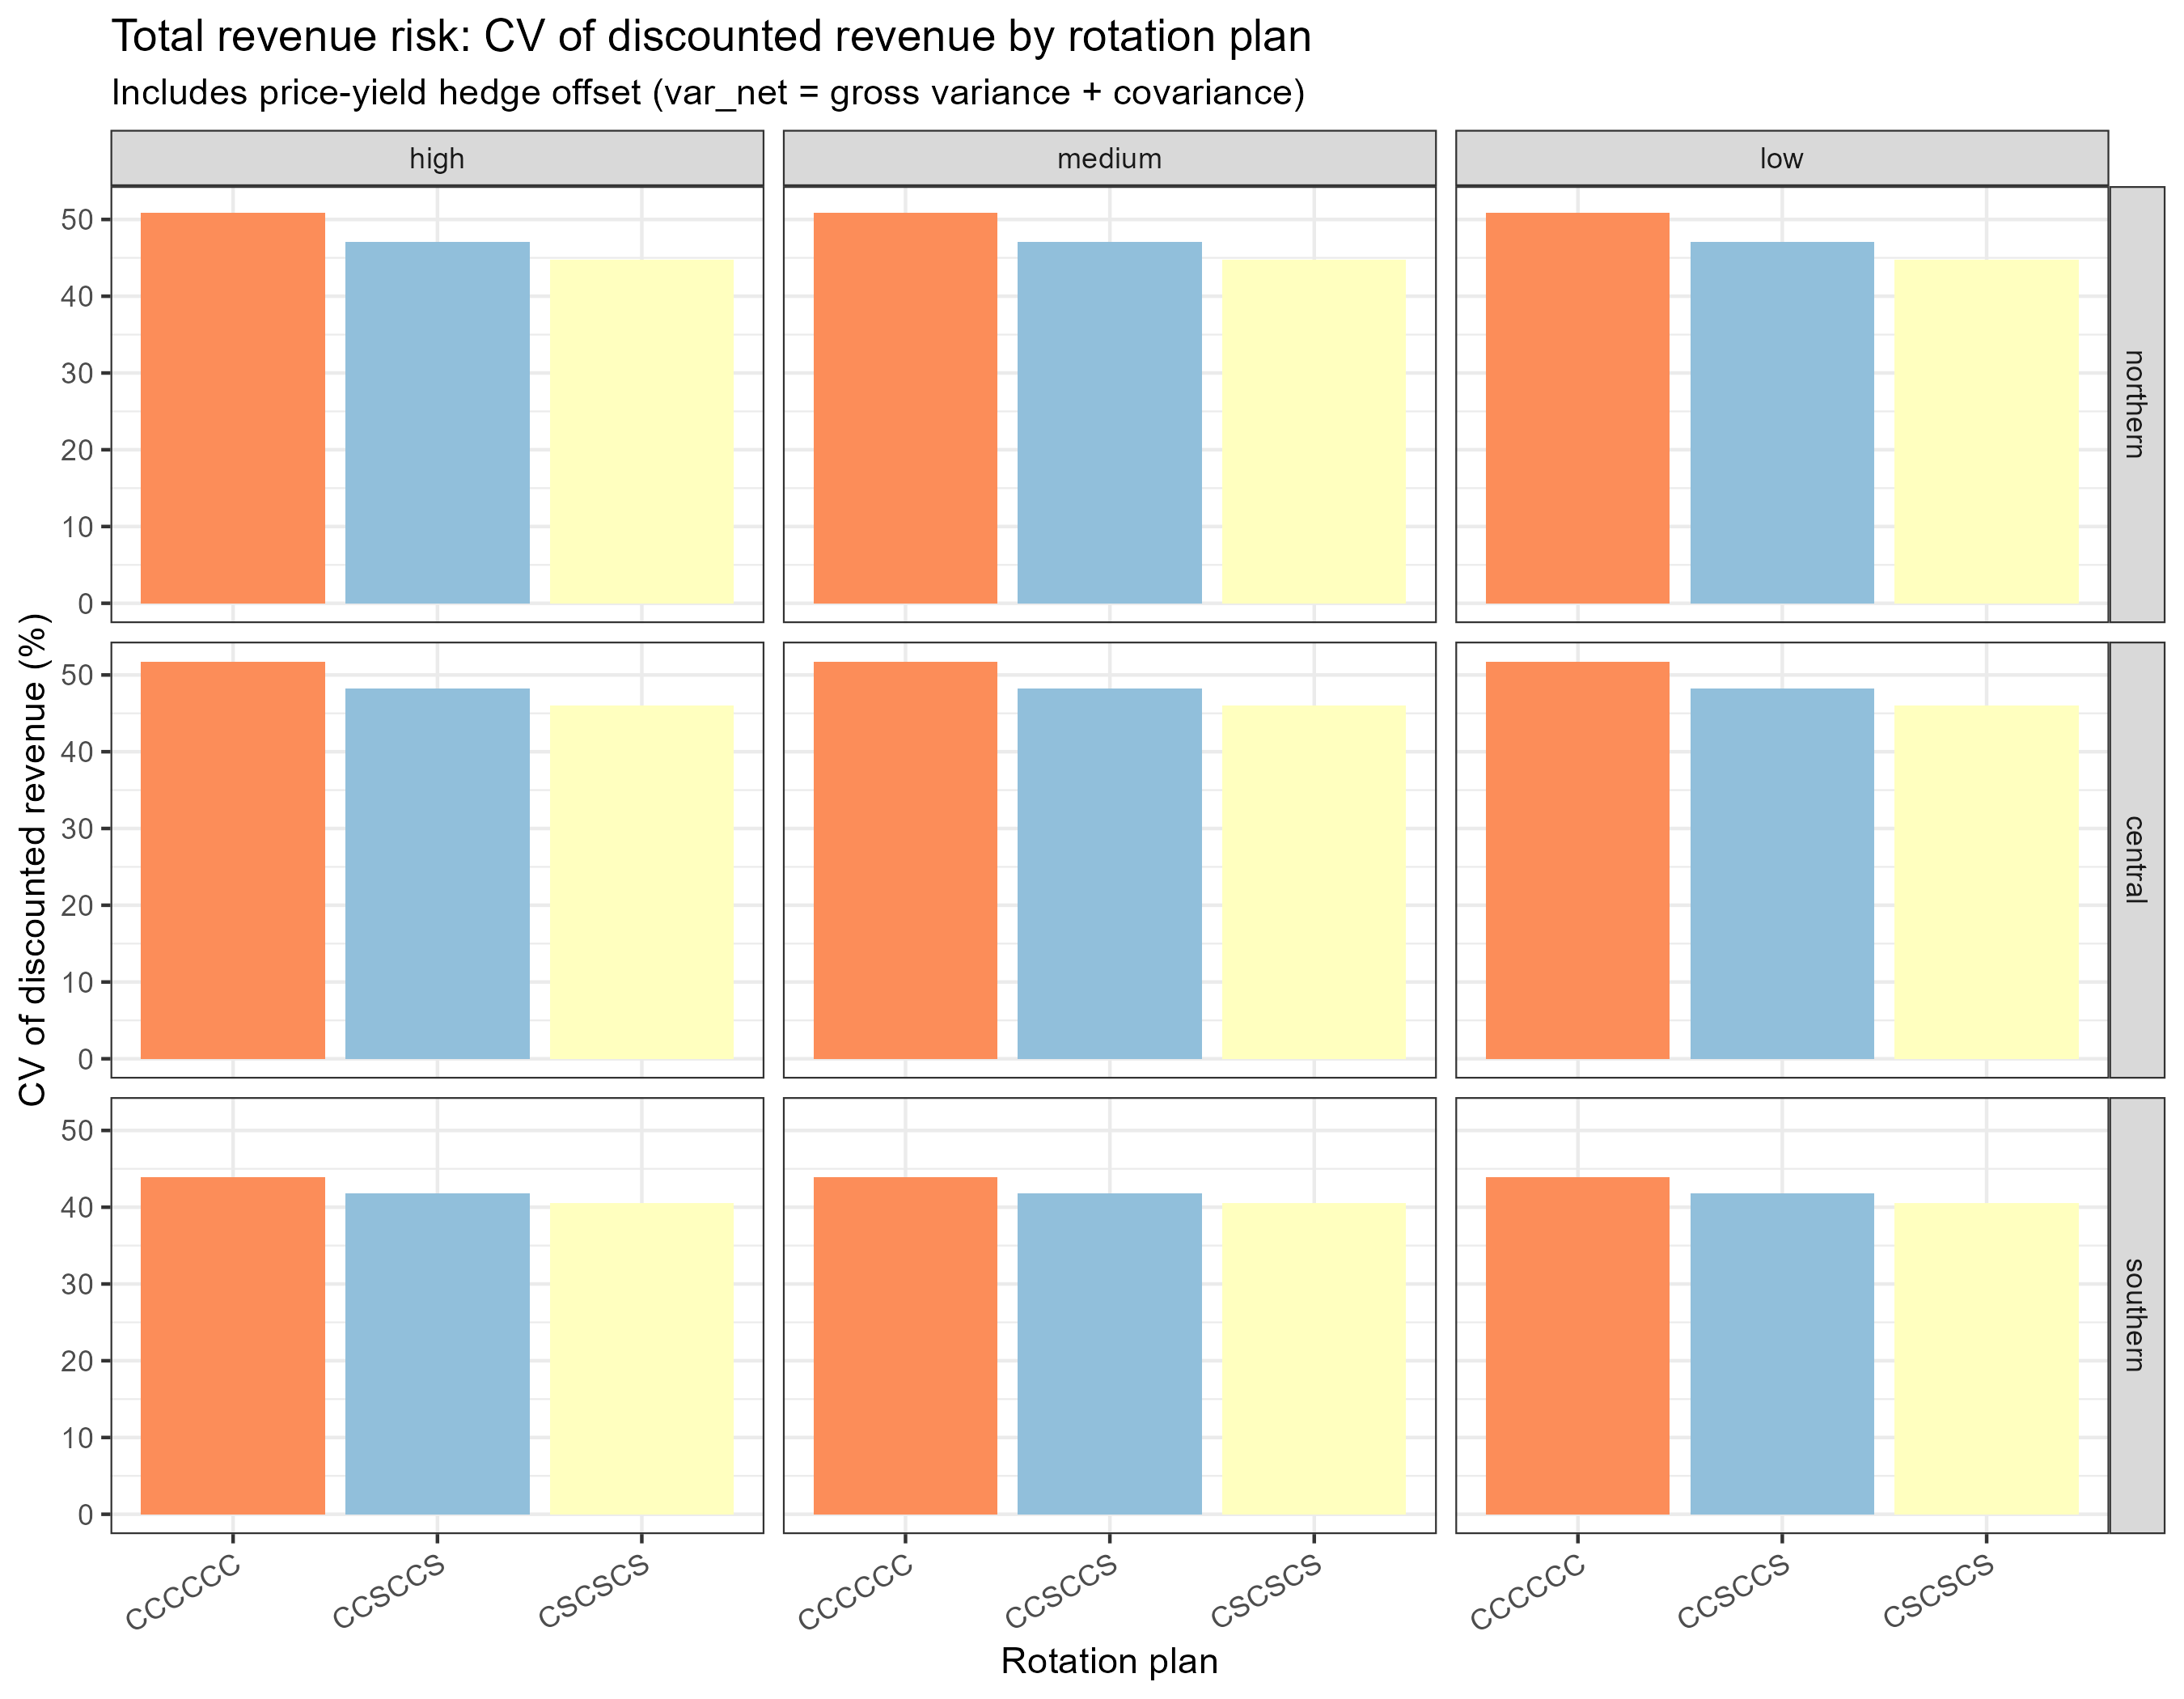
\includegraphics[width=16cm]{figs/fig_revenue_cv.png}
    \caption{Coefficient of variation of discounted six-year revenue by rotation plan, climate region, and productivity zone. The CV includes the price-yield hedge offset (net rather than gross variance).}
    \label{fig:fig_revenue_cv} 
\end{figure}

\subsection{\label{subsec:cum_cf}Cumulative cash flow under the over-limit delinquency rule}
Section \ref{subsec:survival} notes that the simulation is also run under an "over-limit" delinquency rule, in which an event is recorded only if the spring loan demand exceeds the credit ceiling rather than whenever the end-of-year balance is positive. The absolute delinquency rates fall under this stricter rule, naturally, since a positive balance below the credit ceiling no longer counts, but the relative ranking of plans and the sawtooth pattern in per-year hazards both survive.

Figure \ref{fig:fig_p_cf_all} reports the corresponding cumulative net cash flow over the six-year horizon. The median (solid lines) is monotonically increasing in every cell; rotation plans (green, blue) dominate continuous corn (red) by roughly \$100–\$300 per acre by year 6 in the high-productivity zones, and the 10–90 percentile band confirms that the \textbf{lower} tail of cumulative cash flow is also higher under rotation. This is the underlying object that the over-limit delinquency rule conditions on: when the lower tail of cumulative cash is bounded away from zero, the corresponding spring loan demand stays bounded, and the over-limit event becomes rare.

\begin{figure}[H]
    \centering
    \includegraphics[width=16cm]{figs/fig_p_cf_all.png}
    \caption{Median cumulative net cash flow (solid lines) with 10–90 percentile band (shaded), by rotation plan, climate region, and productivity zone.}
    \label{fig:fig_p_cf_all} 
\end{figure}

\subsection{\label{subsec:abs_shapley_vals}Absolute Shapley values}
Section \ref{subsec:shapley} reports the \textit{price share} of Shapley-decomposed delinquency risk, $\phi_P / (\phi_P + \phi_Y)$, which ranges from 92 to 100 percent across the simulation grid. The normalization conceals the underlying \textit{levels}: a 95-percent price share means very different things depending on whether total delinquency risk is 15 percentage points or 55 percentage points.

Figure \ref{fig:fig_shapley_abs} reports the absolute Shapley values $\phi_P$ and $\phi_Y$ in percentage points of delinquency probability, stacked by uncertainty source. The total bar height equals the rotation-plan-specific delinquency probability from Figure 1, decomposed into its price and yield Shapley components. Continuous corn in the central-high cell tops out near 55 percentage points, of which roughly 52 are price-attributable, and 3 are yield-attributable; CSCSCS in southern cells bottoms at 15 percentage points, almost entirely price-driven. The figure makes clear that what changes between high-risk and low-risk cells is the \textit{level} of price risk that survives the rotation's debt-reset mechanism, the yield share is uniformly small in absolute terms across the grid.

\begin{figure}[H]
    \centering
    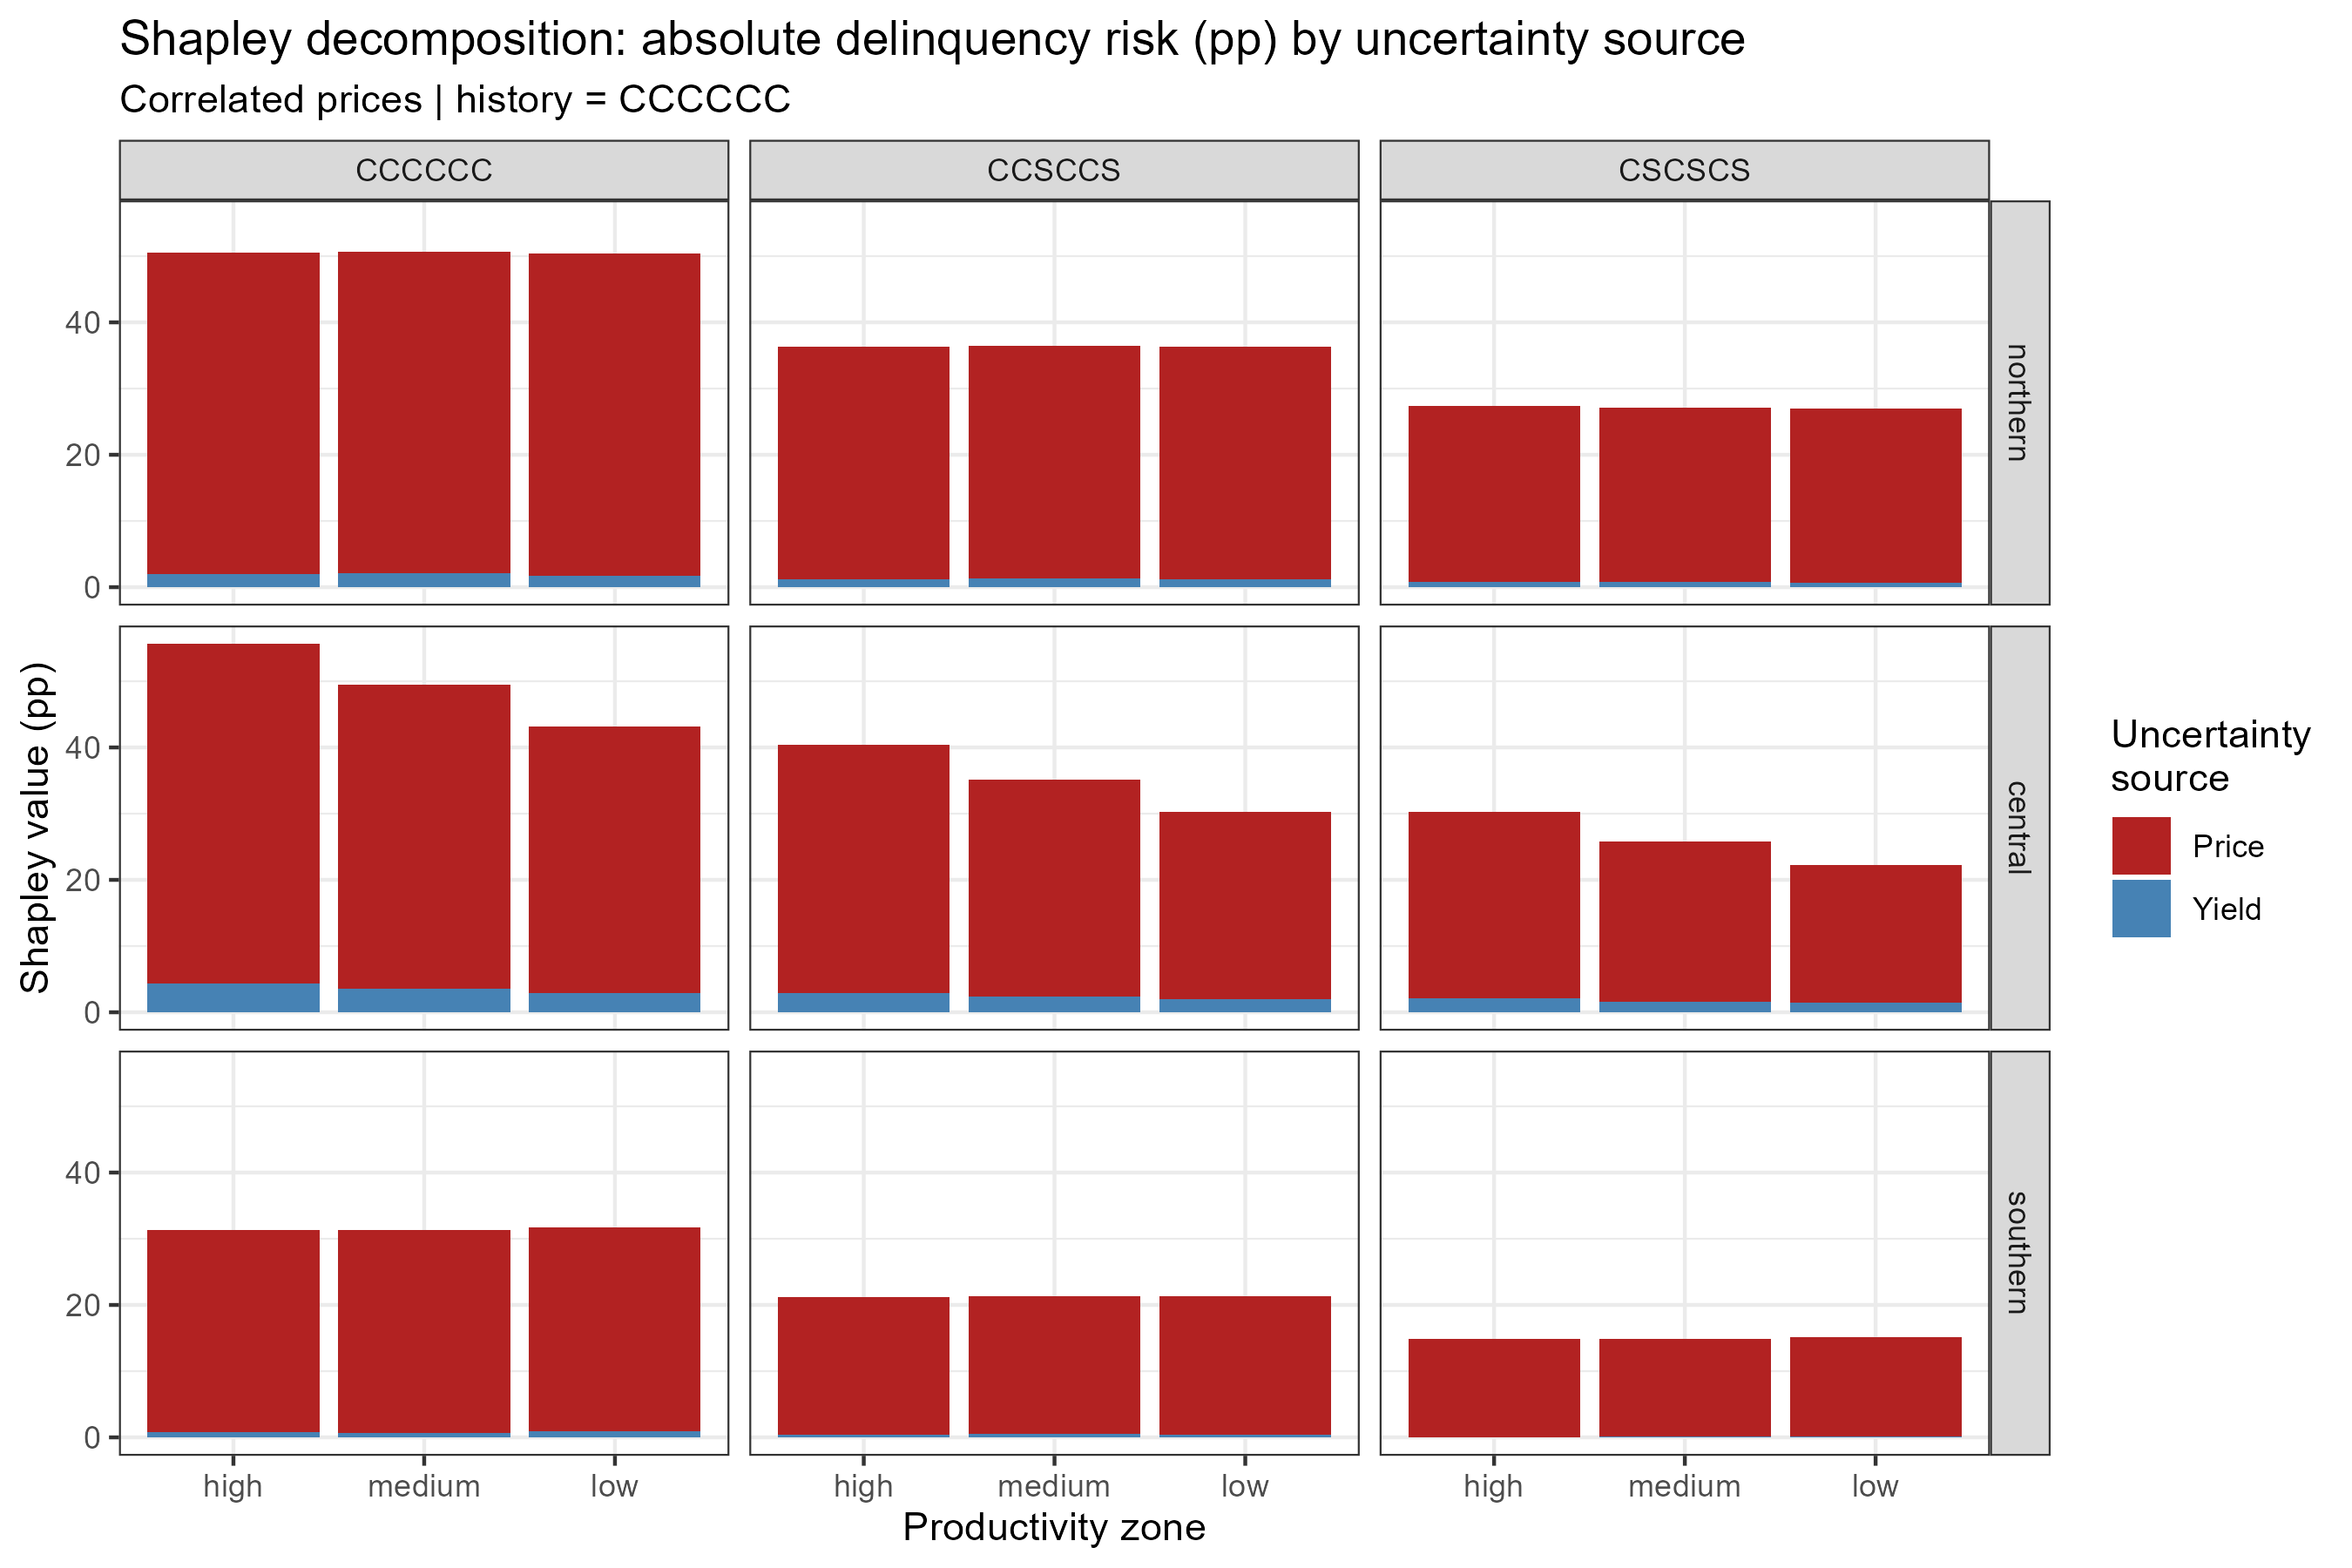
\includegraphics[width=16cm]{figs/fig_shapley_abs.png}
    \caption{Shapley decomposition of six-year delinquency probability into price (red) and yield (blue) components, in percentage points.}
    \label{fig:fig_shapley_abs} 
\end{figure}



\newpage
\bibliographystyle{apalike}
\bibliography{references} 

\end{document}